% !TeX spellcheck = de_CH
%%%%%%%%%%%%%%%%%%%%%%%%%%%%%%%%%%%%%%%%%%%%%%%%%%%%%%%%%%%%%%%%%
%  _____   ____  _____                                          %
% |_   _| /  __||  __ \    Institute of Computitional Physics   %
%   | |  |  /   | |__) |   Zuercher Hochschule Winterthur       %
%   | |  | (    |  ___/    (University of Applied Sciences)     %
%  _| |_ |  \__ | |        8401 Winterthur, Switzerland         %
% |_____| \____||_|                                             %
%%%%%%%%%%%%%%%%%%%%%%%%%%%%%%%%%%%%%%%%%%%%%%%%%%%%%%%%%%%%%%%%%
%
% Project     : BA Welti Keller
% Title       : 
% File        : doc.tex Rev. 00
% Date        : 15.09.2014
% Author      : Tobias Welti
%
%%%%%%%%%%%%%%%%%%%%%%%%%%%%%%%%%%%%%%%%%%%%%%%%%%%%%%%%%%%%%%%%%

%%%%%%%%%%%%%%%%%%%%%%%%%%%%%%%%%%%%%%%%%%%%%%%%%%%%%%%%%%%%%%%%%
%  _____   ____  _____                                          %
% |_   _| /  __||  __ \    Institute of Computitional Physics   %
%   | |  |  /   | |__) |   Zuercher Hochschule Winterthur       %
%   | |  | (    |  ___/    (University of Applied Sciences)     %
%  _| |_ |  \__ | |        8401 Winterthur, Switzerland         %
% |_____| \____||_|                                             %
%%%%%%%%%%%%%%%%%%%%%%%%%%%%%%%%%%%%%%%%%%%%%%%%%%%%%%%%%%%%%%%%%
%
% Project     : Konzept BA Welti Keller
% Title       : 
% File        : header.tex Rev. 00
% Date        : 15.09.2014
% Author      : Tobias Welti
%
%%%%%%%%%%%%%%%%%%%%%%%%%%%%%%%%%%%%%%%%%%%%%%%%%%%%%%%%%%%%%%%%%

\documentclass[twoside,10pt,parskip=half,ngerman]{scrreprt}

%***********************************************************************
% include some libs
%***********************************************************************	
\usepackage[utf8]{inputenc}
\usepackage{listings}
\usepackage{color}
\usepackage{fancyhdr}
\usepackage{rotating}
\usepackage{titlesec}
\usepackage{mathptmx}
\usepackage{todonotes}
 \usepackage{helvet}
%\usepackage[scaled]{uarial}
\renewcommand*\familydefault{\sfdefault} %% Only if the base font of the document is to be sans serif
\usepackage[T1]{fontenc}
\usepackage{ngerman}
\usepackage{textcomp}
\usepackage[squaren]{SIunits}
\usepackage{graphicx}
\usepackage[hyphens]{url}
\usepackage{geometry}
\usepackage[absolute]{textpos}
\usepackage{makeidx}
\usepackage{colortbl}
\usepackage{pdflscape}
\usepackage{pdfpages}
\usepackage{tabularx}
\usepackage{lmodern}
\usepackage{longtable}
\usepackage{array}
\usepackage{float}
\usepackage{scrhack}
\usepackage[plainpages=false]{hyperref}
\usepackage{wallpaper}
\usepackage{hyperref}
\urlstyle{same}

% Glossar
\usepackage[toc,nopostdot,acronyms]{glossaries}
%\usepackage{glossaries-german}
\renewcommand*{\glossaryname}{Glossar}
\renewcommand*{\acronymname}{Abkürzungsverzeichnis}
\setacronymstyle{long-short}
\makeglossaries
\loadglsentries{content/glossar}
%\makenoidxglossaries




% Deutsches Literaturverzeichnis
\usepackage{bibgerm}
% Silbentrennung (Neu-Deutsch)
 \usepackage[ngerman]{babel}
 % Spezialseiten (Literarturverzeichnis, Abbildungsverzeichnis, usw.) in Inhaltsverzeichnis anzeigen
\usepackage[nottoc]{tocbibind}

% Grafiken
%\usepackage[pdftex]{graphicx}
%\usepackage{epsfig}

%***********************************************************************
% various styles
%***********************************************************************	

%create index
\makeindex

%define pagestyle
\pagestyle{fancy}

%use sans-serif font 
%\renewcommand{\familydefault}{\sfdefault}

%define page margin
\geometry{a4paper, top=30mm, left=30mm, right=30mm, bottom=30mm,headsep=10mm,footskip=10mm}

%textpos parameter
\setlength{\TPHorizModule}{30mm}
\setlength{\TPVertModule}{\TPHorizModule}
\textblockorigin{10mm}{10mm} % start everything near the top-left corner
\setlength{\parindent}{0pt}

%horizontal lines for titlepage 
\newcommand{\HRule}{\rule{\linewidth}{0.5mm}}

%reference to source items inlc source number
\newcommand{\srcref}[1]{\nameref{src:#1} \cite{#1}}

%header / footer 
\renewcommand{\headrulewidth}{0.3pt}
\renewcommand{\footrulewidth}{0.3pt}

\fancyhead[LO,RE]{} %clear headings for contents 
\fancyhead[RO,LE]{\nouppercase{\rightmark}} %right odd pages and left even pages
\fancyhead[LO,RE]{\MakeUppercase{\leftmark}} %left odd pages and right even pages
\fancyfoot[LE,RO]{\thepage} %page numbering
\fancyfoot[C]{} %clear centered page numbering 

%define some colors
\definecolor{gray}{rgb}{0.95,0.95,0.95}
\definecolor{darkgray}{rgb}{0.4,0.4,0.4}
%listing colors
\definecolor{lgray}{RGB}{250,250,250}
\definecolor{lgreen}{RGB}{63,127,95}
\definecolor{lred}{RGB}{127,0,85}
\definecolor{lblue}{RGB}{42,0,255}

%***********************************************************************
% listing
%***********************************************************************

\lstset{		
		basicstyle=\small\ttfamily,
		frame=single,
		numbers=left,	
		numberstyle=\tiny,
		%firstnumber=auto,
		numberblanklines=true,
		captionpos=b,
		extendedchars=true,
		float=ht,
		showtabs=false,
		tabsize=2,
		showspaces=false,
		showstringspaces=false,
		breaklines=true,
		%prebreak=\Righttorque,
		backgroundcolor=\color{lgray},
		keywordstyle=\color{lred}\bfseries, 
		commentstyle=\color{lgreen}\ttfamily,
%		morekeywords={printstr, printhexln},
		stringstyle=\color{lblue},
		xleftmargin=0.5cm,
		xrightmargin=0.5cm
}

\lstloadlanguages{C++}

%\lstdefinelanguage{xc}{
%     keywords={printstr, printhexln, attributes, class, classend, do, empty, endif, endwhile, fail, function, functionend, if, implements, in, inherit, inout, not, of, operations, out, return, set, then, types, while, use},
%     keywordstyle=\color{lred}\bfseries,
%     ndkeywords={},
%     ndkeywordstyle=\color{yellow}\bfseries,
%     identifierstyle=\color{black},
%     sensitive=false,
%     comment=[l]{//},
%     commentstyle=\color{lgreen}\ttfamily,
%     string=[l]{"},
%     stringstyle=\color{lblue}\ttfamily
%  }


\begin{document}
\title{Bachelorarbeit (IT)}
\author{Tobias Keller, Tobias Welti}

% !TeX spellcheck = de_CH
%%%%%%%%%%%%%%%%%%%%%%%%%%%%%%%%%%%%%%%%%%%%%%%%%%%%%%%%%%%%%%%%%
%  _____   ____  _____                                          %
% |_   _| /  __||  __ \    Institute of Computitional Physics   %
%   | |  |  /   | |__) |   Zuercher Hochschule Winterthur       %
%   | |  | (    |  ___/    (University of Applied Sciences)     %
%  _| |_ |  \__ | |        8401 Winterthur, Switzerland         %
% |_____| \____||_|                                             %
%%%%%%%%%%%%%%%%%%%%%%%%%%%%%%%%%%%%%%%%%%%%%%%%%%%%%%%%%%%%%%%%%
%
% Project     : BA Welti Keller
% Title       : 
% File        : titlepage.tex Rev. 00
% Date        : 15.09.2014
% Author      : Tobias Welti
%
%%%%%%%%%%%%%%%%%%%%%%%%%%%%%%%%%%%%%%%%%%%%%%%%%%%%%%%%%%%%%%%%%

\begin{titlepage}

% Logo
\ThisTileWallPaper{\paperwidth}{\paperheight}{images/logos/InES.pdf} % {}images/logos/*.pdf}
% Wählen Sie aus folenden pdf Files: ICP, IDP, IEFE, IMES, IMPE, IMS, INE, InES, InIT, KSR, SoE, ZAMP, ZAV, ZIL, ZPP, ZSN

\begin{minipage}[b]{0.117\textwidth}
\hskip 0.05cm
\end{minipage}
\begin{minipage}[b]{0.91\textwidth}
\begin{tiny}.\end{tiny}\vskip 2.8cm
	{\huge
	
	% Projekt Name
	\textbf{\underline{Bachelorarbeit}}
	
	% Projekt Titel
	Messstation zur Registrierung von Geschiebe-Bewegungen im Fluss
	\vskip 0.5cm}
	
	\begin{minipage}[b]{0.27\textwidth}
	\hrule\vskip 0.5cm
		\textbf{Autoren}\\
		\\
	\end{minipage}
	\begin{minipage}[b]{0.03\textwidth}
	\hskip 0.5cm
	\end{minipage}
	\begin{minipage}[b]{0.7\textwidth}
	\hrule\vskip 0.5cm
		Tobias Keller\\
		Tobias Welti\\
	\end{minipage}
	
	\begin{minipage}[b]{0.27\textwidth}
	\hrule\vskip 0.5cm
		\textbf{Betreuer}\\
		\\
	\end{minipage}
	\begin{minipage}[b]{0.03\textwidth}
	\hskip 0.5cm
	\end{minipage}
	\begin{minipage}[b]{0.7\textwidth}
	\hrule\vskip 0.5cm
		Prof. Hans-Joachim Gelke, Dipl. El. Ing. FH\\
		ZHAW Institute for Embedded Systems\\
	\end{minipage}
	
	\begin{minipage}[b]{0.27\textwidth}
	\hrule\vskip 0.5cm
		\textbf{Partner}\\
		\\
	\end{minipage}
	\begin{minipage}[b]{0.03\textwidth}
	\hskip 0.5cm
	\end{minipage}
	\begin{minipage}[b]{0.7\textwidth}
	\hrule\vskip 0.5cm
	  Carlos Rodrigo Wyss\\
		Eidg. Forschungsanstalt für Wald, Schnee und Landschaft WSL\\
	\end{minipage}
	
	\begin{minipage}[b]{0.27\textwidth}
	\hrule\vskip 0.5cm
		\textbf{Datum}
	\end{minipage}
	\begin{minipage}[b]{0.03\textwidth}
	\hskip 0.5cm
	\end{minipage}
	\begin{minipage}[b]{0.7\textwidth}
	\hrule\vskip 0.5cm
		\today
	\end{minipage}
\end{minipage}
\vskip 0.5cm

\end{titlepage}

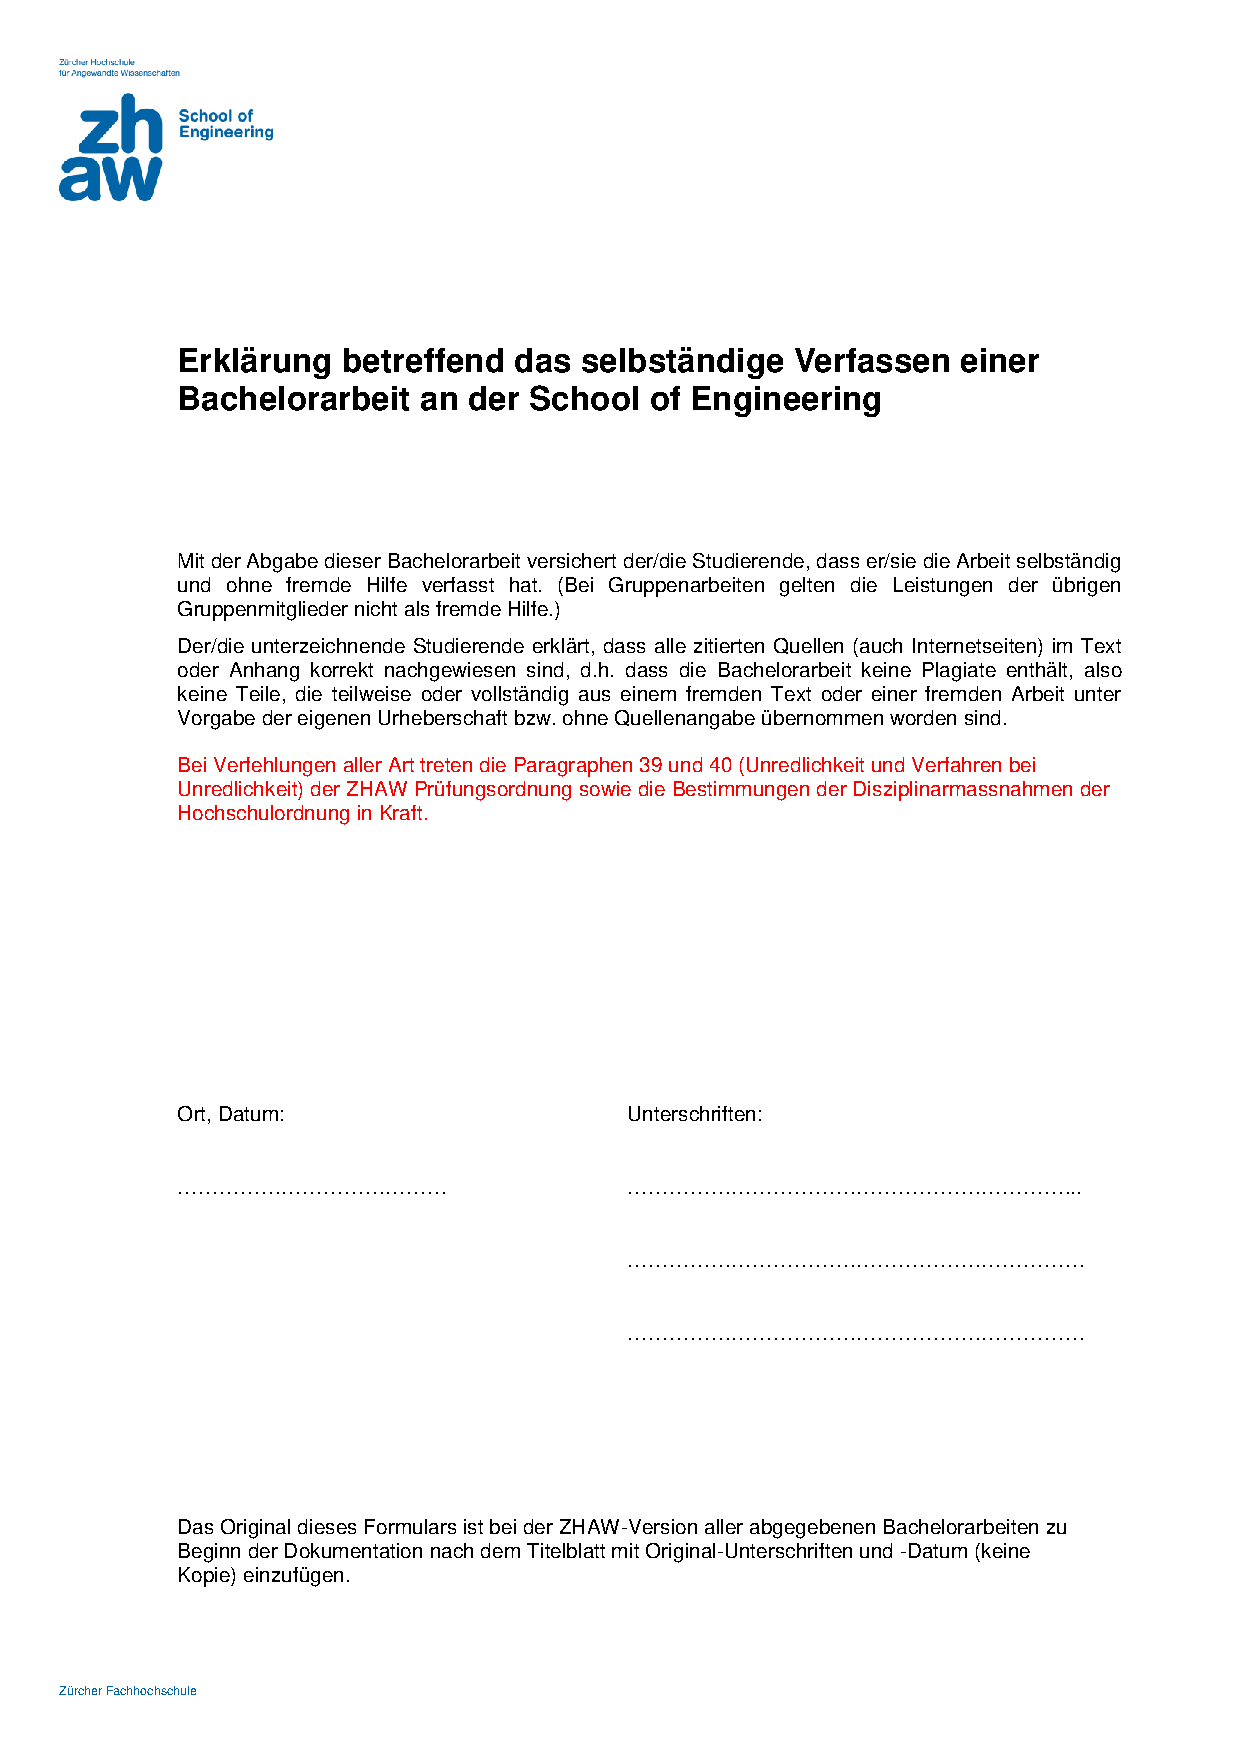
\includepdf{images/Erklaerung_BA.pdf}
% !TeX spellcheck = de_CH
%%%%%%%%%%%%%%%%%%%%%%%%%%%%%%%%%%%%%%%%%%%%%%%%%%%%%%%%%%%%%%%%%
%  _____   ____  _____                                          %
% |_   _| /  __||  __ \    Institute of Computitional Physics   %
%   | |  |  /   | |__) |   Zuercher Hochschule Winterthur       %
%   | |  | (    |  ___/    (University of Applied Sciences)     %
%  _| |_ |  \__ | |        8401 Winterthur, Switzerland         %
% |_____| \____||_|                                             %
%%%%%%%%%%%%%%%%%%%%%%%%%%%%%%%%%%%%%%%%%%%%%%%%%%%%%%%%%%%%%%%%%
%
% Project     : BA Welti Keller
% Title       : 
% File        : vorwort.tex Rev. 00
% Date        : 15.09.2014
% Author      : Tobias Welti
%
%%%%%%%%%%%%%%%%%%%%%%%%%%%%%%%%%%%%%%%%%%%%%%%%%%%%%%%%%%%%%%%%%

\chapter*{Vorwort}\label{chap.vorwort}
Durch eine Studienkollegin kamen wir im Sommer 2013 mit Bruno Fritschi von der Eidgenössischen Forschungsanstalt für Wald, Schnee und Landschaft (WSL) in Kontakt und konnten uns von ihm einige äusserst interessante Ideen für Bachelorarbeiten im Bereich Embedded Systems vorstellen lassen. Ziemlich schnell waren wir uns einig, dass die Entwicklung eines Bussystems zur Messung von Geschiebetransport nach einer spannenden und herausfordernden Aufgabe tönt und entschlossen uns, diese als Bachelorarbeit anzugehen. Wie wir feststellen mussten, ist die Planung und Implementation eines ganzen Systems eine ziemliche Herausforderung, zumal wir beide bis jetzt nur wenig Erfahrung in diesem Bereich gesammelt hatten. Dank dem fachlichen Know-how von Bruno Fritschi und Hans Gelke konnten wir zum Schluss einen funktionierenden Prototyp erstellen, der zumindest die Machbarkeit dieser Lösung bestätigt. Es gibt aber durchaus noch einige Punkte, die man verbessern oder erweitern muss, bevor man von einem finalen Produkt sprechen kann.

\setcounter{page}{1}
\include{content/kontakt}


%Inhaltsverzeichnis
\tableofcontents
\listoftodos
\newpage


%Kapitel
%\setcounter{page}{1}
%\pagenumbering{arabic}

% !TeX spellcheck = de_CH
%%%%%%%%%%%%%%%%%%%%%%%%%%%%%%%%%%%%%%%%%%%%%%%%%%%%%%%%%%%%%%%%%
%  _____   ____  _____                                          %
% |_   _| /  __||  __ \    Institute of Computitional Physics   %
%   | |  |  /   | |__) |   Zuercher Hochschule Winterthur       %
%   | |  | (    |  ___/    (University of Applied Sciences)     %
%  _| |_ |  \__ | |        8401 Winterthur, Switzerland         %
% |_____| \____||_|                                             %
%%%%%%%%%%%%%%%%%%%%%%%%%%%%%%%%%%%%%%%%%%%%%%%%%%%%%%%%%%%%%%%%%
%

% Project     : Pflichtenheft BA Welti Keller
% Title       : 
% File        : einleitung.tex Rev. 00
% Date        : 15.09.2014
% Author      : Tobias Welti
%
%%%%%%%%%%%%%%%%%%%%%%%%%%%%%%%%%%%%%%%%%%%%%%%%%%%%%%%%%%%%%%%%%

\chapter{Einleitung}\label{chap.einleitung}



\section{Ausgangslage}\label{sec.ausgangslage}
Die Eidg. Forschungsanstalt für Wald, Schnee und Landschaft (WSL) betreibt Messstationen zur Registrierung von Geschiebe-Bewegungen im Fluss mittels Geophonen, die unter Stahlplatten montiert sind. Diese Platten sind in einer Betonkonstruktion eingelassen, um sie im Flussbett zu fixieren. Die Geophone sind über Kabel mit einem Auswertungs-Rechner (Embedded PC) verbunden, der die Signale auswertet. Die baulichen Massnahmen für die Installation der Sensoren, der Auswertungsstation sowie der Stromversorgung sind sehr teuer. 


\section{Aufgabenstellung}\label{sec.aufgabenstellung}
Im Rahmen dieser Bachelorarbeit soll eine Lösung erarbeitet werden, um zukünftige Installationen günstiger zu machen. Da solche Messanlagen an sehr vielen Orten auf der ganzen Welt aufgebaut werden, kann durch eine Vereinfachung der Installation viel Aufwand gespart werden. 

Die Projektidee stammt von Bruno Fritschi (WSL). Sein Vorschlag sieht vor, die aufgezeichneten Signale direkt am Sensor auszuwerten und nur die gewünschten Ereignisse zu übertragen und zu speichern. Somit könnten die Daten über ein Bussystem übertragen werden und der Auswertungsrechner bräuchte weniger Leistung.

Dank der Bustopologie ist das Messsystem weniger komplex und kann einfacher installiert werden. Denkbar wäre die Integration in einer Gummimatte anstelle der Stahl- und Betonkonstruktion, da viel weniger Leitungen nötig sind.

Ziel der Arbeit ist die Entwicklung der Auswertungshardware und des Bussystems. Die Qualität der gemessenen Signale soll mindestens erhalten werden. Die Auswertungsalgorithmen sind nicht Bestandteil der Arbeit und werden vom WSL zur Verfügung gestellt.

Die von der bisherigen Anlage gemachten Messdaten enthalten die Dauer und Intensität jedes Aufschlags (Ereignis) auf der Sensorplatte, sowie die Anzahl Ausschläge (Peaks) pro Aufschlag. Pro Minute wird ein Histogramm über die Intesitäten der Peaks gebildet und abgespeichert.

Denkbar wäre es, einen Prototyp für Vergleichsmessungen im Erlenbach (Alptal, SZ) an einer bestehenden Schwelle zu implementieren.

\subsection{Musskriterien}
\begin{itemize}
\item Die Anlage zeichnet den Geschiebetransport im Bachbett auf. Die bisherige Aufzeichnungsrate von 10'000 Messpunkten pro Sekunde soll nicht unterschritten werden.
\item Die Anlage liefert eine minütliche Zusammenfassung über die Ereignisse an jedem Sensor. Diese Zusammenfassung enthält die Anzahl, Dauer und Intensität der einzelnen Ereignisse sowie ein Histogramm über die Intensitätsverteilung.
\item Die Messstation ist fähig, mindestens zehn Sensoren zu betreiben und ihre Messignale aufzuzeichnen.
\item Es ist möglich, die kompletten Rohdaten von einem Sensor über eine Dauer von 30 Minuten aufzuzeichnen. Während einer solchen Messung dürfen die anderen Sensoren ihre Messung einstellen.
\item Die Sensoren können über bis zu fünfzehn Meter im Bachbett verteilt sein.
\item Die Leistungsaufnahme der Anlage beim Betrieb von 10 Sensoren ist kleiner als zehn Watt.
\item Die Datenaufzeichnung erfolgt in einem eigens entwickelten Datenlogger.
\item Am Datenlogger kann ein Laptop angeschlossen werden, um Kontrollparameter der Messanlage zu setzen und um den Status der Anlage abzufragen.
\item Die erfassten Messdaten werden im Datenlogger auf einer Speicherkarte gespeichert. Dies ermöglicht ein einfaches Abholen der Daten im Feld, indem die Speicherkarte ausgetauscht wird.
\end{itemize}
\subsection{Wunschkriterien}
\begin{itemize}
\item Die Anlage liefert für jedes Ereignis die Rohdaten in voller zeitlicher Auflösung.
\item Der Sensoraufbau ermöglicht es, die Sensoren in einer Elastomerplatte zu verpacken. Die Elastomerplatte kann ohne Betonkonstruktion im Bachbett verankert werden.
\item Am Datenlogger kann ein Laptop angeschlossen werden, um die erfassten Messdaten herunterzuladen.
\end{itemize}
\subsection{Abgrenzungskriterien}
\begin{itemize}
\item Es würde den Rahmen dieser Arbeit sprengen, die Messeinheiten zur Produktreife zu bringen. Es wird lediglich aufgezeigt, wie solche Messeinheiten realisiert werden könnten.
\item Eine Testinstallation in einem Bach ist nicht möglich. Allenfalls kann in der Versuchsanstalt für Wasserbau, Hydrologie und Glaziologie der ETH Zürich ein kleiner Testlauf stattfinden.
\item
\end{itemize}

% !TeX spellcheck = de_CH
%%%%%%%%%%%%%%%%%%%%%%%%%%%%%%%%%%%%%%%%%%%%%%%%%%%%%%%%%%%%%%%%%
%  _____   ____  _____                                          %
% |_   _| /  __||  __ \    Institute of Computitional Physics   %
%   | |  |  /   | |__) |   Zuercher Hochschule Winterthur       %
%   | |  | (    |  ___/    (University of Applied Sciences)     %
%  _| |_ |  \__ | |        8401 Winterthur, Switzerland         %
% |_____| \____||_|                                             %
%%%%%%%%%%%%%%%%%%%%%%%%%%%%%%%%%%%%%%%%%%%%%%%%%%%%%%%%%%%%%%%%%
%
% Project     : BA Welti Keller
% Title       : 
% File        : aufgabenstellung.tex Rev. 00
% Date        : 15.09.2014
% Author      : Tobias Welti
%
%%%%%%%%%%%%%%%%%%%%%%%%%%%%%%%%%%%%%%%%%%%%%%%%%%%%%%%%%%%%%%%%%

\chapter{Aufgabenstellung}\label{chap.aufgabenstellung}

Die offizielle Aufgabenstellung befindet sich im Anhang \ref{app.aufgabenstellung}.

\section{Aufgabenstellung}\label{sec.aufgabenstellung}
Im Rahmen dieser Bachelorarbeit soll eine Lösung erarbeitet werden, um zukünftige Installationen günstiger zu machen. Da solche Messanlagen an sehr vielen Orten auf der ganzen Welt aufgebaut werden, kann durch eine Vereinfachung der Installation viel Aufwand gespart werden. 

Die Projektidee stammt von Bruno Fritschi (WSL). Sein Vorschlag sieht vor, die aufgezeichneten Signale direkt am \gls{sensor} auszuwerten und nur die gewünschten \gls{ereignis}-Daten zu übertragen und zu speichern. Somit könnten die Daten über ein \gls{bussys} übertragen werden und der Rechner für die Sammlung der Daten bräuchte weniger Rechenleistung.

Dank der Bustopologie kommt das Messsystem mit weniger Leitungen aus und kann einfacher installiert werden. Denkbar wäre die Integration in einer Elastomerplatte anstelle der Stahl- und Betonkonstruktion, da viel weniger Leitungen nötig sind. Die Elastomerplatte könnte einfacher im Bachbett verankert werden.

Ziel der Arbeit ist die Entwicklung der Auswertungshardware und des \gls{bussys}s. Die Qualität der gemessenen Signale soll mindestens erhalten werden. Die Auswertungsalgorithmen sind nicht Bestandteil der Arbeit und werden vom WSL zur Verfügung gestellt.

Die von der bisherigen Anlage gemachten Messdaten enthalten die Dauer und Intensität jedes Aufschlags (\gls{ereignis}) auf der Sensorplatte, sowie die Anzahl Ausschläge (Peaks) pro Aufschlag. Pro Minute wird ein Histogramm über die Intesitäten der Peaks gebildet und abgespeichert.

Denkbar wäre es, einen Prototyp für Vergleichsmessungen im Erlenbach (Alptal, SZ) an einer bestehenden Schwelle zu implementieren.


\subsection{Musskriterien}
\begin{itemize}
\item Die Anlage zeichnet den Geschiebetransport im Bachbett auf. Die bisherige Aufzeichnungsrate von 10'000 Messpunkten pro Sekunde soll nicht unterschritten werden.
\item Die Anlage liefert eine minütliche Zusammenfassung über die \glspl{ereignis} an jedem \gls{sensor}. Diese Zusammenfassung enthält die Anzahl, Dauer und Intensität der einzelnen \glspl{ereignis} sowie ein Histogramm über die Intensitätsverteilung.
\item Die Messstation ist fähig, mindestens zehn \glspl{sensor} zu betreiben und ihre Messignale aufzuzeichnen.
\item Es ist möglich, die kompletten Rohdaten von einem \gls{sensor} über eine Dauer von 30 Minuten aufzuzeichnen. Während einer solchen Messung dürfen die anderen \glspl{sensor} ihre Messung einstellen.
\item Die \glspl{sensor} können über bis zu fünfzehn Meter im Bachbett verteilt sein.
\item Die Leistungsaufnahme der Anlage beim Betrieb von 10 \glspl{sensor} ist kleiner als zehn Watt.
\item Die Datenaufzeichnung erfolgt in einem eigens entwickelten \gls{logger}.
\item Am \gls{logger} kann ein Laptop angeschlossen werden, um Kontrollparameter der Messanlage zu setzen und um den Status der Anlage abzufragen.
\item Die erfassten Messdaten werden im \gls{logger} auf einer Speicherkarte gespeichert. Dies ermöglicht ein einfaches Abholen der Daten im Feld, indem die Speicherkarte ausgetauscht wird.
\end{itemize}
\subsection{Wunschkriterien}
\begin{itemize}
\item Die Anlage liefert für jedes \gls{ereignis} die Rohdaten in voller zeitlicher Auflösung.
\item Der Sensoraufbau ermöglicht es, die \glspl{sensor} in einer Elastomerplatte zu verpacken. Die Elastomerplatte kann ohne Betonkonstruktion im Bachbett verankert werden.
\item Am \gls{logger} kann ein Laptop angeschlossen werden, um die erfassten Messdaten herunterzuladen.
\end{itemize}
\subsection{Abgrenzungskriterien}
\begin{itemize}
\item Es würde den Rahmen dieser Arbeit sprengen, die Messeinheiten zur Produktreife zu bringen. Es wird lediglich aufgezeigt, wie solche Messeinheiten realisiert werden könnten.
\item Eine Testinstallation in einem Bach ist nicht möglich. Allenfalls kann in der Versuchsanstalt für Wasserbau, Hydrologie und Glaziologie der ETH Zürich ein kleiner Testlauf stattfinden.
\item
\end{itemize}


% !TeX spellcheck = de_CH
%%%%%%%%%%%%%%%%%%%%%%%%%%%%%%%%%%%%%%%%%%%%%%%%%%%%%%%%%%%%%%%%%
%  _____   ____  _____                                          %
% |_   _| /  __||  __ \    Institute of Computitional Physics   %
%   | |  |  /   | |__) |   Zuercher Hochschule Winterthur       %
%   | |  | (    |  ___/    (University of Applied Sciences)     %
%  _| |_ |  \__ | |        8401 Winterthur, Switzerland         %
% |_____| \____||_|                                             %
%%%%%%%%%%%%%%%%%%%%%%%%%%%%%%%%%%%%%%%%%%%%%%%%%%%%%%%%%%%%%%%%%
%
% Project     : BA Welti Keller
% Title       : 
% File        : vorgehen.tex Rev. 00
% Date        : 15.09.2014
% Author      : Tobias Welti
%
%%%%%%%%%%%%%%%%%%%%%%%%%%%%%%%%%%%%%%%%%%%%%%%%%%%%%%%%%%%%%%%%%

\chapter{Vorgehen}\label{chap.vorgehen}

% !TeX spellcheck = de_CH
% !TeX spellcheck = de_CH
%%%%%%%%%%%%%%%%%%%%%%%%%%%%%%%%%%%%%%%%%%%%%%%%%%%%%%%%%%%%%%%%%
%  _____   ____  _____                                          %
% |_   _| /  __||  __ \    Institute of Computational Physics   %
%   | |  |  /   | |__) |   Zuercher Hochschule Winterthur       %
%   | |  | (    |  ___/    (University of Applied Sciences)     %
%  _| |_ |  \__ | |        8401 Winterthur, Switzerland         %
% |_____| \____||_|                                             %
%%%%%%%%%%%%%%%%%%%%%%%%%%%%%%%%%%%%%%%%%%%%%%%%%%%%%%%%%%%%%%%%%
%
% Project     : BA Welti Keller
% Title       : 
% File        : funktionale.tex Rev. 00
% Date        : 15.09.2014
% Author      : Tobias Welti
%
%%%%%%%%%%%%%%%%%%%%%%%%%%%%%%%%%%%%%%%%%%%%%%%%%%%%%%%%%%%%%%%%%

\thispagestyle{empty}
\chapter{Funktionale Anforderungen}\label{chap.funktionale}
\section{\gls{logger} (F1\ldots)}


\subsection{F110 Busmaster}
Der \gls{logger} übernimmt die Kontrolle des \gls{bussys}. Bei Inbetriebnahme des Systems tastet der \gls{logger} den Bus nach \glspl{sensoreinh} ab und erteilt jeder \gls{sensoreinh} eine eindeutige Identifikationsnummer (ID). Die ID des \gls{logger}s soll so gewählt werden, dass er jederzeit Priorität hat, auf den Bus zu schreiben.


\subsection{F120 Sensorerkennung}
Die angeschlossenen \glspl{sensor} werden vom \gls{logger} erkannt und mit einer ID versehen. Anhand der ID wird die Priorität bei der Datenübertragung festgelegt und der \gls{sensor} identifiziert. Ein Sensor, der bereits am System angeschlossen war, erhält wieder die gleiche \gls{id}, sofern die Konfigurationsdatei nicht gelöscht wurde.


\subsection{F130 Uhrzeit}
Der \gls{logger} verfügt über eine interne Uhr, um die \glspl{ereignis} in den Dateien mit einem lesbaren Zeitstempel zu versehen.


\subsection{F140 \gls{timestamp} verteilen}
Der \gls{logger} sendet ein Signal an alle \glspl{sensoreinh}, dass der Zeitstempel (\gls{timestamp}) neu gestellt werden soll. Ab dann beziehen sich die \gls{timestamp}s auf die Dauer seit dem jetzigen Zeitpunkt.


\subsection{F160 Schnittstelle zum Steuerrechner}
Der \gls{logger} bietet eine Schnittstelle, an der ein Steuerrechner (Laptop, \gls{pc}) angeschlossen werden kann. Über diese Schnittstelle kann der Betrieb der ganzen Anlage gesteuert werden.


\subsection{F170 Steuerung Betriebsmodus}
Der Betriebsmodus der \glspl{sensor} wird vom \gls{logger} aus gesteuert: Wie viele und welche Art von Daten gesammelt werden soll und ob alle \glspl{sensor} oder nur bestimmte aktiv sein sollen. \\
Folgende Betreibsmodi sind verfügbar:
\begin{itemize}
\item Normaler Modus: Alle \glspl{sensor} übermitteln die verarbeiteten Ereignisdaten. Zeitpunkt, Intensität, Dauer und Anzahl Ausschläge jedes \gls{ereignis} werden gespeichert.
\item Detaillierter Modus: Alle \glspl{sensor} übermitteln die verarbeiteten Ereignisdaten sowie die gesamten Messdaten für die Dauer des \gls{ereignis}.
\item Rohdatenmodus: Ein \gls{sensor} übermittelt kontinuierlich Rohdaten, die anderen \glspl{sensor} werden vorübergehend abgeschaltet.
\end{itemize}


\subsection{F180 Daten sammeln}
Der \gls{logger} fragt in regelmässigen Abständen bei den \glspl{sensoreinh} an, ob Ereignisdaten zur Übertragung bereit sind. Diese übermitteln die vorliegenden Ereignisdaten.


\subsection{F190 Daten speichern}
Die Daten werden vom \gls{logger} auf einer Speicherkarte in Dateien abgelegt. Nach entsprechenden Befehlen vom Steuerrechner kann die Karte entfernt und ausgetauscht werden, um die Daten abzuholen.


\section{\gls{sensoreinh} (F4\ldots)}


\subsection{F410 Ereignisdetektion}
Die \gls{sensoreinh} liest den \gls{sensor} mit einer definierten \gls{fs} aus und wertet die Messdaten aus. Der Prozessor erkennt \glspl{ereignis} anhand definierter Kriterien. Zu jedem \gls{ereignis} werden folgende Daten gespeichert: Zeitpunkt (\gls{timestamp}), Dauer, Anzahl Peaks und höchster Peak. In einem zweiten Betriebsmodus können alle Messpunkte während einem \gls{ereignis} gespeichert werden.


\subsection{F430 Datenübertragung}
Die \gls{sensoreinh} übermittelt die Ereignisdaten über das \gls{bussys} an den \gls{logger}.


\subsection{F450 Rohdatenaufzeichnung}
In einem Sondermodus werden alle Messpunkte gespeichert und über das \gls{bussys} an den \gls{logger} übertragen. In diesem Betriebsmodus kann darf auch nur eine \gls{sensoreinh} aktiv sein, die anderen werden auf Standby geschaltet.



% !TeX spellcheck = de_CH
%%%%%%%%%%%%%%%%%%%%%%%%%%%%%%%%%%%%%%%%%%%%%%%%%%%%%%%%%%%%%%%%%
%  _____   ____  _____                                          %
% |_   _| /  __||  __ \    Institute of Computitional Physics   %
%   | |  |  /   | |__) |   Zuercher Hochschule Winterthur       %
%   | |  | (    |  ___/    (University of Applied Sciences)     %
%  _| |_ |  \__ | |        8401 Winterthur, Switzerland         %
% |_____| \____||_|                                             %
%%%%%%%%%%%%%%%%%%%%%%%%%%%%%%%%%%%%%%%%%%%%%%%%%%%%%%%%%%%%%%%%%
%
% Project     : Pflichtenheft BA Welti Keller
% Title       : 
% File        : nichtfunktionale.tex Rev. 00
% Date        : 15.09.2014
% Author      : Tobias Welti
%
%%%%%%%%%%%%%%%%%%%%%%%%%%%%%%%%%%%%%%%%%%%%%%%%%%%%%%%%%%%%%%%%%

\thispagestyle{empty}
\chapter{Nichtfunktionale Anforderungen}\label{chap.nichtfunktionale}

\begin{itemize}
\item Die gesamte Messstation soll eine geringere Leistungsaufnahme haben als eine aktuelle Messstation mit Geophonen. Für zehn Geophone sind dies zur Zeit zehn Watt.

\item Die Installation soll weniger bauliche Massnahmen erfordern als eine aktuelle Messstation mit Geophonen.

\item Die erfassten Ereignisdaten sollen mehr Details enthalten als mit den bisherigen Installationen.

\item Sensoreinheiten müssen wasserdicht verpackt werden können.
\
\end{itemize}
% !TeX spellcheck = de_CH
%%%%%%%%%%%%%%%%%%%%%%%%%%%%%%%%%%%%%%%%%%%%%%%%%%%%%%%%%%%%%%%%%
%  _____   ____  _____                                          %
% |_   _| /  __||  __ \    Institute of Computitional Physics   %
%   | |  |  /   | |__) |   Zuercher Hochschule Winterthur       %
%   | |  | (    |  ___/    (University of Applied Sciences)     %
%  _| |_ |  \__ | |        8401 Winterthur, Switzerland         %
% |_____| \____||_|                                             %
%%%%%%%%%%%%%%%%%%%%%%%%%%%%%%%%%%%%%%%%%%%%%%%%%%%%%%%%%%%%%%%%%
%
% Project     : BA Welti Keller
% Title       : 
% File        : grundlagen.tex Rev. 00
% Date        : 15.09.2014
% Author      : Tobias Welti
%
%%%%%%%%%%%%%%%%%%%%%%%%%%%%%%%%%%%%%%%%%%%%%%%%%%%%%%%%%%%%%%%%%

% Kapitel rausgenommen

\chapter{Grundlagen}\label{chap.grundlagen}
\todo{Grundlagen: entweder aus anderen Kapiteln zusammentragen oder das Kapitel streichen}
\todo{etwas über signalerfassung, (aufwand hilbert etc.), mems?}
% !TeX spellcheck = de_CH
%%%%%%%%%%%%%%%%%%%%%%%%%%%%%%%%%%%%%%%%%%%%%%%%%%%%%%%%%%%%%%%%%
%  _____   ____  _____                                          %
% |_   _| /  __||  __ \    Institute of Computitional Physics   %
%   | |  |  /   | |__) |   Zuercher Hochschule Winterthur       %
%   | |  | (    |  ___/    (University of Applied Sciences)     %
%  _| |_ |  \__ | |        8401 Winterthur, Switzerland         %
% |_____| \____||_|                                             %
%%%%%%%%%%%%%%%%%%%%%%%%%%%%%%%%%%%%%%%%%%%%%%%%%%%%%%%%%%%%%%%%%
%
% Project     : BA Welti Keller
% Title       : 
% File        : hardware.tex Rev. 00
% Date        : 15.09.2014
% Author      : Tobias Welti
%
%%%%%%%%%%%%%%%%%%%%%%%%%%%%%%%%%%%%%%%%%%%%%%%%%%%%%%%%%%%%%%%%%

\chapter{Hardware-Konzept}\label{chap.hardware}



\section{Hardware-Architektur}\label{sec.hw_arch}

Anhand der funktionalen Vorgaben für die Messstation werden der \gls{logger}, die \gls{sensoreinh} und das Bussytem im folgenden genauer spezifiziert und die Komponenten ausgewählt.

\subsection{Datenlogger}
Der \gls{logger} sammelt die Daten der \glspl{sensoreinh} über das \gls{bussys} ein und speichert sie ab. Dafür benötigt er das \gls{bussys}, einen Mikroprozessor, internen Speicher und ein leicht auswechselbares Speichermedium. Ausserdem soll über eine Schnittstelle ein Computer angeschlossen werden können, um den Betrieb der Messstation zu steuern. Der \gls{logger} wird in einem wasserdichten Gehäuse untergebracht. Für den Austausch des Speichermediums wäre eine verschraubbare Öffnung denkbar.

\begin{figure}[H]
	\centering
		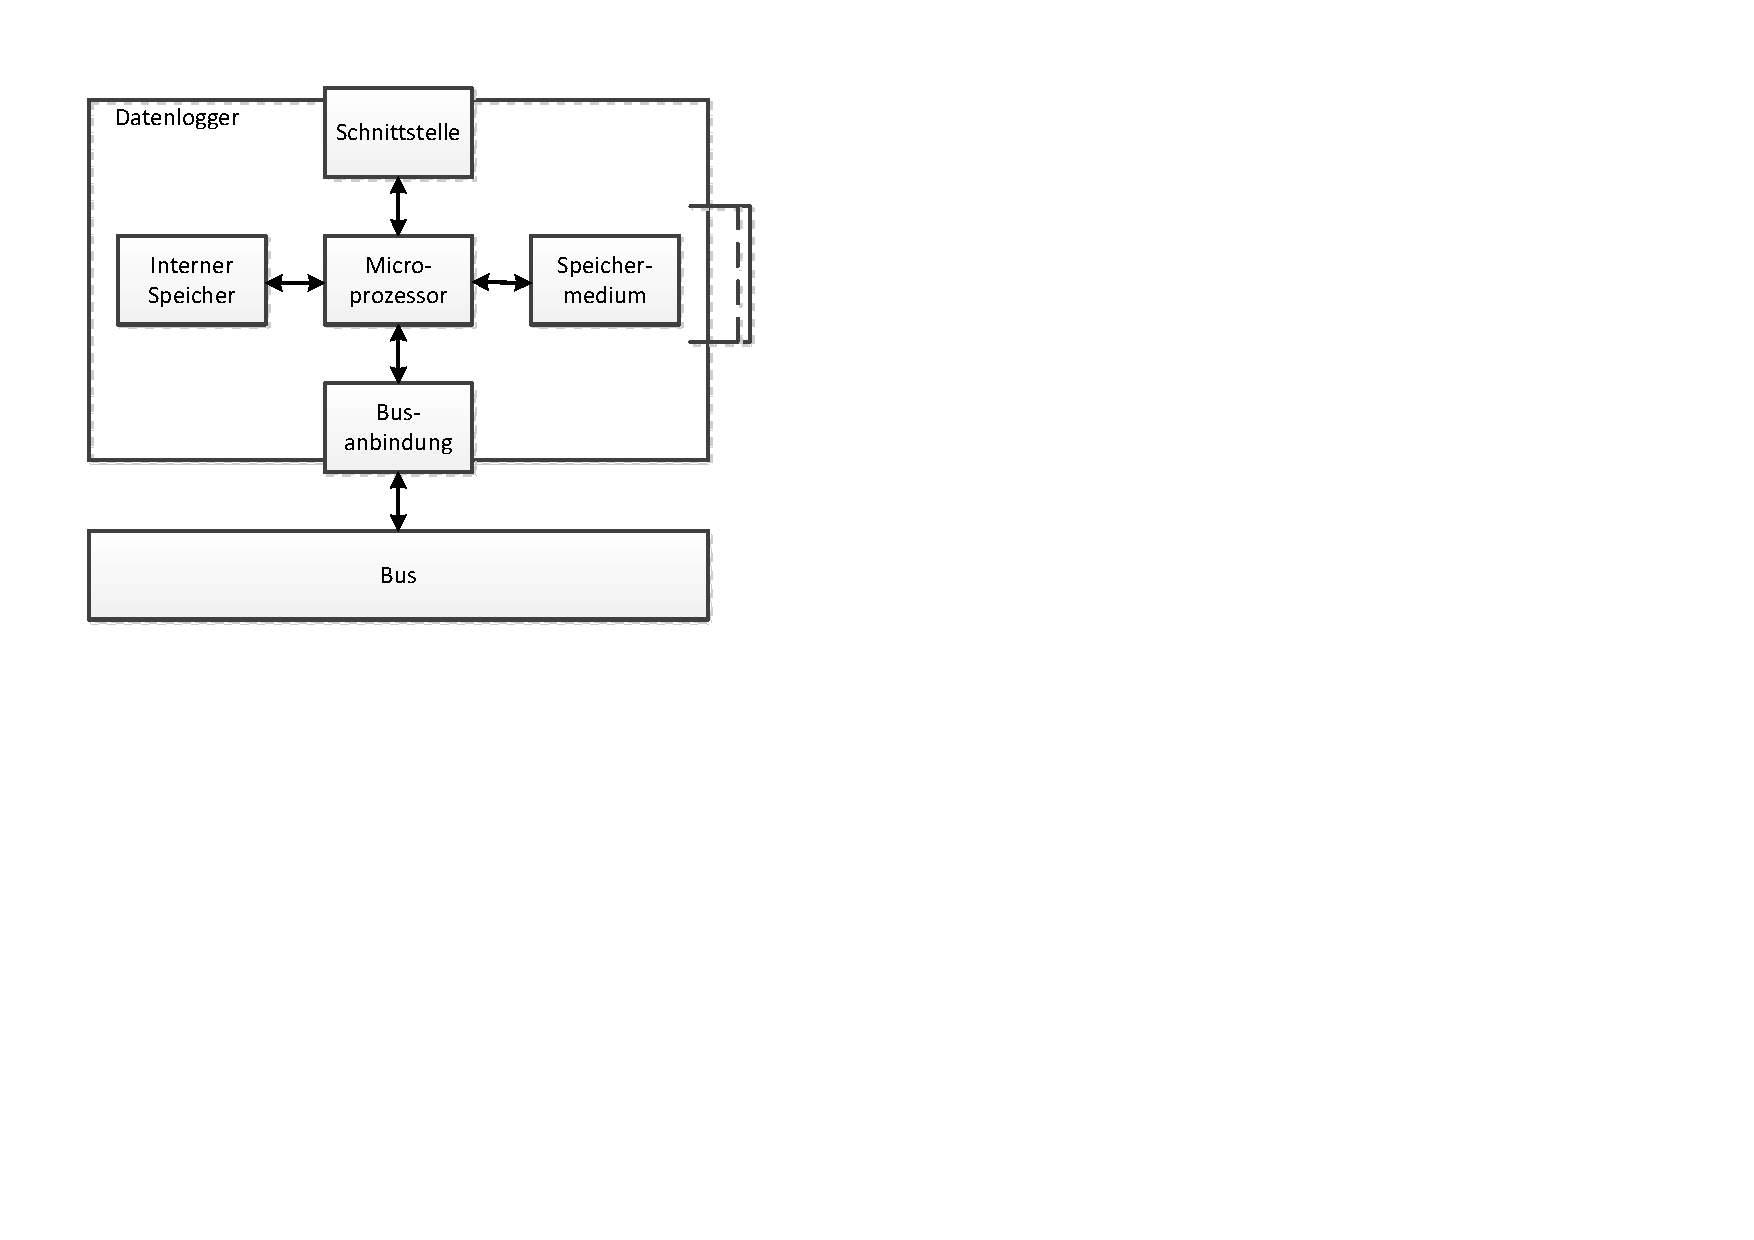
\includegraphics[width=0.8\textwidth]{images/visio/hardwarekonzept_logger.pdf}
	\caption{Hardwarekonzept des \gls{logger}s.}
	\label{fig.hwkonzept_logger}
\end{figure}

\subsection{Sensoreinheit}
Die \gls{sensoreinh} benötigt einen Beschleunigungssensor, um die Einschläge von Geschiebe zu messen. Über einen Analog-Digital-Wandler (ADC) werden die Messsignale digitalisiert. Die gemessenen Signale werden von einem Mikroprozessor verarbeitet, im internen Speicher zwischengespeichert und über das \gls{bussys} an den \gls{logger} übertragen.

\begin{figure}[H]
	\centering
		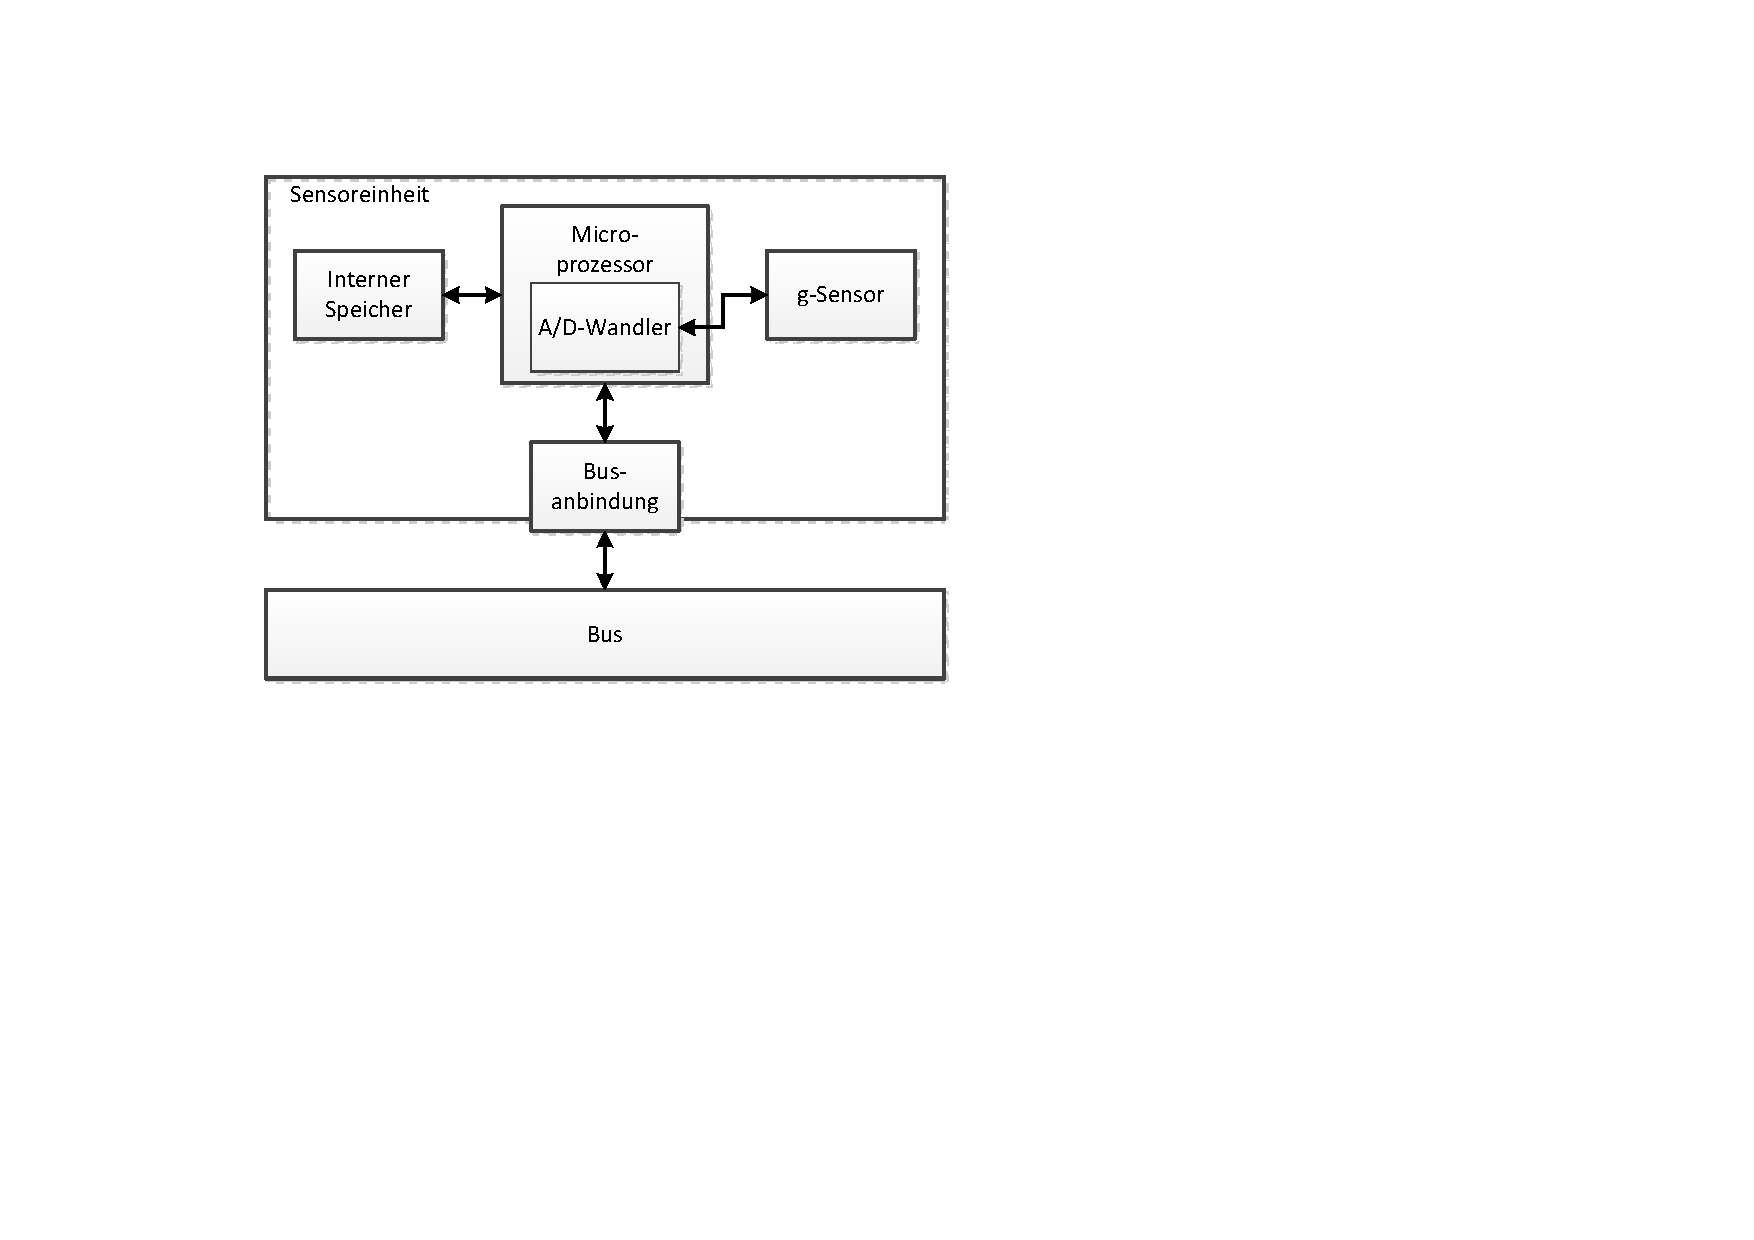
\includegraphics[width=0.8\textwidth]{images/visio/hardwarekonzept_sensor.pdf}
	\caption{Hardwarekonzept der \gls{sensoreinh}.}
	\label{fig.hwkonzept_sensor}
\end{figure}

\subsection{\gls{bussys}}
Das \gls{bussys} muss die Daten und Befehle zwischen \gls{logger} und \glspl{sensoreinh} übertragen. Die Reichweite des \gls{bussys}s muss genügen, um alle Komponenten der Messinstallation zu verbinden. Die Datenbandbreite muss die Übertragung der Messresultate aller \glspl{sensor} erlauben.


\section{Komponentenauswahl}

\subsection{Mikroprozessor}
Bei der Auswahl des Mikroprozessors werden folgende Kriterien berücksichtigt:

\begin{itemize}
\item Rechenleistung genügend für allfällige zusätzliche Anforderungen.
\item Analog-Digital-Wandler mit genügender Abtastrate und Auflösung.
\item Digitaler Signal Prozessor integriert für die Verarbeitung der Messdaten.
\item Ein-/Ausgänge für das \gls{bussys}.
\item Ein-/Ausgänge für den externen Speicher.
\item möglichst geringer Stromverbrauch.
\end{itemize}

\todo{Tabelle verschiedener uCs zum Vergleich}

\subsection{Bus-System}
Anhand folgender Kriterien wurde ein \gls{bussys} ausgewählt:

\begin{itemize}
\item Übertragungsbandbreite genügend für fortlaufende Übertragung von Rohdaten einer \gls{sensoreinh}.
\item Reichweite mindestens 20 Meter.
\item Robust gegenüber äusseren Einflüssen.
\item Mindestens zwanzig Busteilnehmer möglich.
\end{itemize}

\begin{table}
\begin{tabular}{|l|l|l|l|l|}
\hline  & \textbf{Bitrate}      & \textbf{Distanz} & \textbf{Clients} & \textbf{Besonderheiten}\\ 
\hline \textbf{CAN} & \begin{minipage}{2cm}
1 MBit/s\\ 125 kBit/s
\end{minipage} & \begin{minipage}{1.5cm}40 m\\500 m\end{minipage} & > 20 & \begin{minipage}{6cm}
\mbox{ }\\+ Collision Detection (CD) umgehen mit Polling durch Master.\\
+ Bei synchronem CAN wird CD durch ID gelöst.\\
+ CAN Controller sendet Interrupt Request bei erhaltener Nachricht.\\
\end{minipage} \\ 
\hline \textbf{SPI} & ..100 MBit/s & < 1 m & \begin{minipage}{1cm}
slave select
\end{minipage} & \begin{minipage}{6cm}
\mbox{ }\\- Pro Client eine Slave Select Leitung\\
- Daisy Chain $\Rightarrow $alle MC beschäftigt.\\
- Bei Ausfall eines MC ganzer Bus unterbrochen.\\
\end{minipage} \\ 
\hline \textbf{RS485} & \begin{minipage}{2cm}
35 MBit/s\\100 kBit/s
\end{minipage} & \begin{minipage}{1.5cm}
10 m\\1200 m
\end{minipage} & >32 & \begin{minipage}{6cm}
\mbox{ }\\- Master am besten in der Mitte des Bus $\Rightarrow$ ungünstig.\\
- Braucht 2..4 Drähte (bei Full Duplex)\\
- braucht pull-up und pull-down Widerstände $\Rightarrow$ mehr Leistungsaufnahme.\\
\end{minipage} \\ 
\hline \textbf{Ethernet} & 100 MBit/s & 100 m & > 20 & \begin{minipage}{6cm}
\mbox{ }\\+ Stromversorgung bei Power over Ethernet (PoE) integriert.\\
- kein Bus sondern allenfalls Daisychain.\\
- bei Daisychain kein PoE möglich.\\
\end{minipage} \\ 
\hline \textbf{Feldbus} &  &  &  & \begin{minipage}{6cm}
\mbox{ }\\ist eine Familie von Bussen, z.B. CAN-Bus\\
\end{minipage} \\ 
\hline \textbf{I2C} & 0.4..5 Mbit/s & wenige Meter & < 20 & \begin{minipage}{6cm}
\mbox{ }\\nur für kurze Distanzen, Bitrate nimmt rasch ab.\\
\end{minipage}\\
\hline 
\end{tabular}
\caption{Entscheidungsmatrix für die Auswahl des \gls{bussys}s.}
\label{table.bussystem}
\end{table} 

In Tabelle \ref{table.bussystem} sind die Eigenschaften diverser \glspl{bussys} aufgeführt.

\paragraph{Kommentare}
SPI und I2C sind nur für kurze Distanzen geeignet und sind deshalb keine Option.
Die Verwendung von Ethernet zur Datenübertragung würde zwei Schnittstellen auf jeder \gls{sensoreinh} voraussetzen, um die \glspl{sensor} hintereinander zusammenzuhängen (Daisychain). Jedes Paket müsste vom Microcontroller weitergeleitet werden, wenn es für einen anderen Empfänger bestimmt ist. Dies führte zu einer zusätzlichen Belastung der Microcontroller. Stromversorgung über Ethernet ist mit PowerOverEthernet (PoE) zwar möglich, erfordert aber spezielle Geräte zur Speisung über den Stecker des Datenkabels. Dies verunmöglicht eine Daisychain mit PoE, neben dem Datenkabel wäre noch ein Kabel für die Stromversorgung notwendig.

\paragraph{Vergleich CAN-Bus und RS485}
\todo{Kriterienliste RS485/CAN einfügen, Lit-Referenz auf White Paper von IXXAT}
CAN und RS: Stecker nicht definiert => wasserdichte Stecker einfach zu finden.

\paragraph{Entscheidung}
CAN-Bus erfüllt alle Kriterien und erlaubt es, den Busmaster am Ende des Bus zu platzieren. Dies ist ein Vorteil gegenüber RS485, wo der Master in der Mitte platziert werden sollte. CAN-Bus bietet bereits Kollisionserkennung und Fehlererkennung, während dies bei RS485 in der Software gelöst werden muss. Für CAN-Bus sind Bus-Treiber (Transceiver) erhältlich, die mit hohen Spannungen umgehen können, was das \gls{bussys} robuster gegenüber Umwelteinflüssen macht. Die Grösse der Datenpakete ist bei CAN-Bus auf 8 Byte begrenzt, bei RS485 werden die Datenpakete über die Software frei definiert, was ein klarer Vorteil von RS485 darstellt. Insgesamt überwiegen die Vorteile von CAN-Bus klar. 



\subsection{Speichermedium}
\paragraph{Kriterien} Das externe Speichermedium soll möglichst klein sein, wenig Stromverbrauch haben und einfach auswechselbar sein. Bei Inaktivität sollte das Medium wenn möglich keinen Strom verbrauchen. Für einen mehrwöchigen unabhängigen Betrieb einer Messstation muss genügend Speicherkapazität bereitgestellt werden.

\paragraph{Datenmenge} Pro \gls{sensor} werden bei hohem Geschiebeaufkommen maximal hundert \glspl{ereignis} pro Sekunde erwartet. Ein solches Geschiebeaufkommen stellt jedoch die Ausnahme dar. Ein \gls{ereignis} benötigt je nach verlangtem Detailgrad und Dauer des \gls{ereignis}ses 10..90 Byte Speicherplatz. Für den normalen Betriebsmodus werden 50 Byte/\gls{ereignis} gerechnet, bei 5 \glspl{ereignis}n pro Sekunde. Damit ergibt sich eine Datenrate von 250 Byte/s, die es pro \gls{sensor} abzuspeichern gilt. Mit zehn \glspl{sensor} im Einsatz müssen 2.5 kByte/s gespeichert werden. 

\paragraph{Unabhängige Betriebsdauer} Pro Gigabyte Speicherplatz können 111 Stunden Daten für zehn \glspl{sensor} gespeichert werden. Bei hohem Geschiebeaufkommen mit zwanzig mal mehr \glspl{ereignis}n bleiben immer noch 5 Stunden Aufzeichnungszeit pro Gigabyte. Begnügt man sich mit weniger Details, reichen fallen pro \gls{sensor} in zehn Sekunden rund 400 Byte Daten an. Bei dieser Datenrate reicht ein Gigabyte für rund 700 Stunden. Auch bei hohem Geschiebeaufkommen kann die Anlage mehrere Tage an Daten speichern. 

\paragraph{Kapazität} Heute sind Speichermedien mit Kapazitäten bis über 128 GB erhältlich, so dass die Detailrate kein entscheidendes Kriterium mehr darstellt.

\paragraph{Datentransfer} Für den Transfer der Daten aus dem \gls{logger} auf einen Computer gibt es grundsätzlich zwei Varianten. Entweder man liest die Daten über eine Schnittstelle auf den Computer aus, oder man tauscht das Speichermedium aus. Das Auslesen via Schnittstelle benötigt zusätzlich Strom, das Wechseln des Speichermediums setzt einen mehr oder weniger komfortablen und trotzdem wasserdichten Zugang zum Medium voraus. Da heute Speichermedien mit kleinem Platzbedarf erhältlich sind, könnte ein solcher Zugang recht einfach mit einem Schraubverschluss realisiert werden.

\paragraph{Vergleich} In Tabelle \ref{table.speichermedium} werden verschiedene Speichermedien miteinander verglichen. In der Spalte 'Breite' ist aufgelistet, wie gross eine Öffnung mindestens sein muss, um das Speichermedium wechseln zu können. 'Pins' gibt an, wie viele Leitungen für den Anschluss des Mediums am Microcontroller nötig sind. Der Stromverbrauch in Klammern ist für den Standby-Modus des Speichermediums.

\begin{table}
\begin{tabular}{|l|l|l|l|l|}
	\hline
	                      & \textbf{Breite} & \textbf{Pins} & \textbf{Stromverbrauch} & \textbf{Bemerkungen}        \\ \hline
	\textbf{SD-Card}      & 24 mm           & 9             & 20..100 mA (0.2 mA)     & 4 bit breiter serieller Bus \\ \hline
	\textbf{CompactFlash} & 43 mm           & 50            & max. 70 mA (k.A.)       & paralleler Bus              \\ \hline
	\textbf{USB-Stick}    & min. 12 mm      & 4             & typ. 70 mA (k.A.) &  \\ \hline
\end{tabular} 
\caption{Entscheidungsmatrix zur Auswahl des Speichermediums.}
\label{table.speichermedium}
\end{table} 

\todo{Literatur-Referenzen in Tabelle \ref{table.speichermedium}}


\paragraph{Entscheid} Für einen verschraubbaren Verschluss ist die CompactFlash-Karte zu breit, das Gehäuse würde dadurch sehr gross werden. Die SD-Karte und der USB-Stick sind vergleichbar in der Grösse. Von der SD-Karte sind auch kleinere Varianten erhältlich. Eine Öffnung für den Austausch des Speichermediums kann eine gewisse Grösse ohnehin nicht unterschreiten, damit hineingegriffen werden kann. Da die SD-Karte im Standby den geringeren Stromverbrauch hat, wird der \gls{logger} mit einem SD-Kartenleser ausgestattet.

\subsection{Sensor}
\todo{Sensorauswahl beschreiben}

\subsection{Schnittstelle}
\todo{Schnittstellenauswahl beschreiben}



\section{Komponenten}
\todo{Texten}
\subsection{Cortex M4 Mikroprozessor}

\todo{Texten}
\subsubsection{Flash Speicher}

\todo{Texten}
\subsubsection{SDRAM}

\todo{Texten}

\subsection{Beschleunigungs-Sensor}

\todo{Texten}
\subsection{CAN Bus}

\todo{Texten}
\subsubsection{CAN Transceiver}

\todo{Texten}

\subsection{SD Karte}

\todo{Texten}
\subsection{UART Schnittstelle}

\todo{Texten}
\section{\gls{logger}}

\todo{Texten}
\begin{figure}[H]
	\centering
		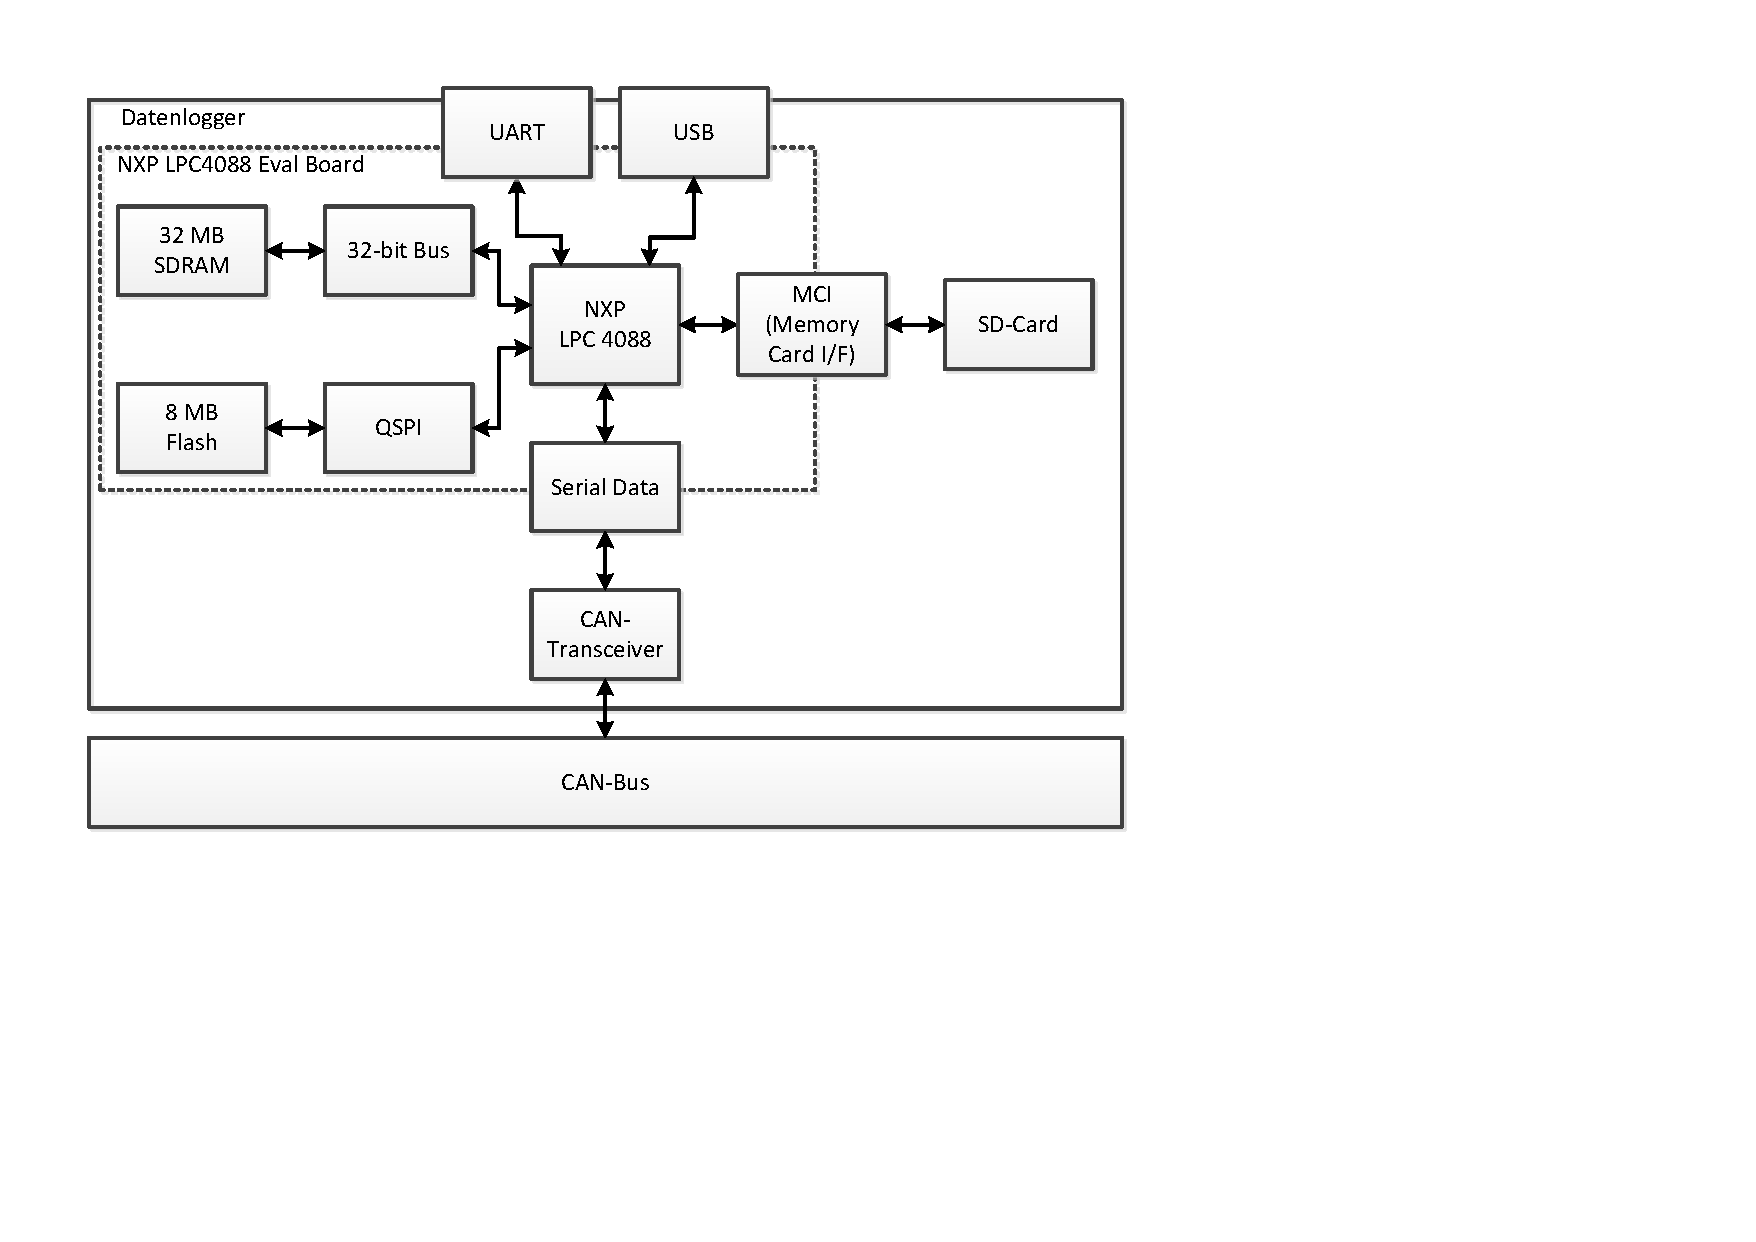
\includegraphics[width=0.8\textwidth]{images/visio/hardware_logger.pdf}
	\caption{Schematischer Hardware-Aufbau des \gls{logger}s.}
	\label{fig.hw_logger}
\end{figure}



\section{Sensoreinheit}

\todo{Texten}
\begin{figure}[H]
	\centering
		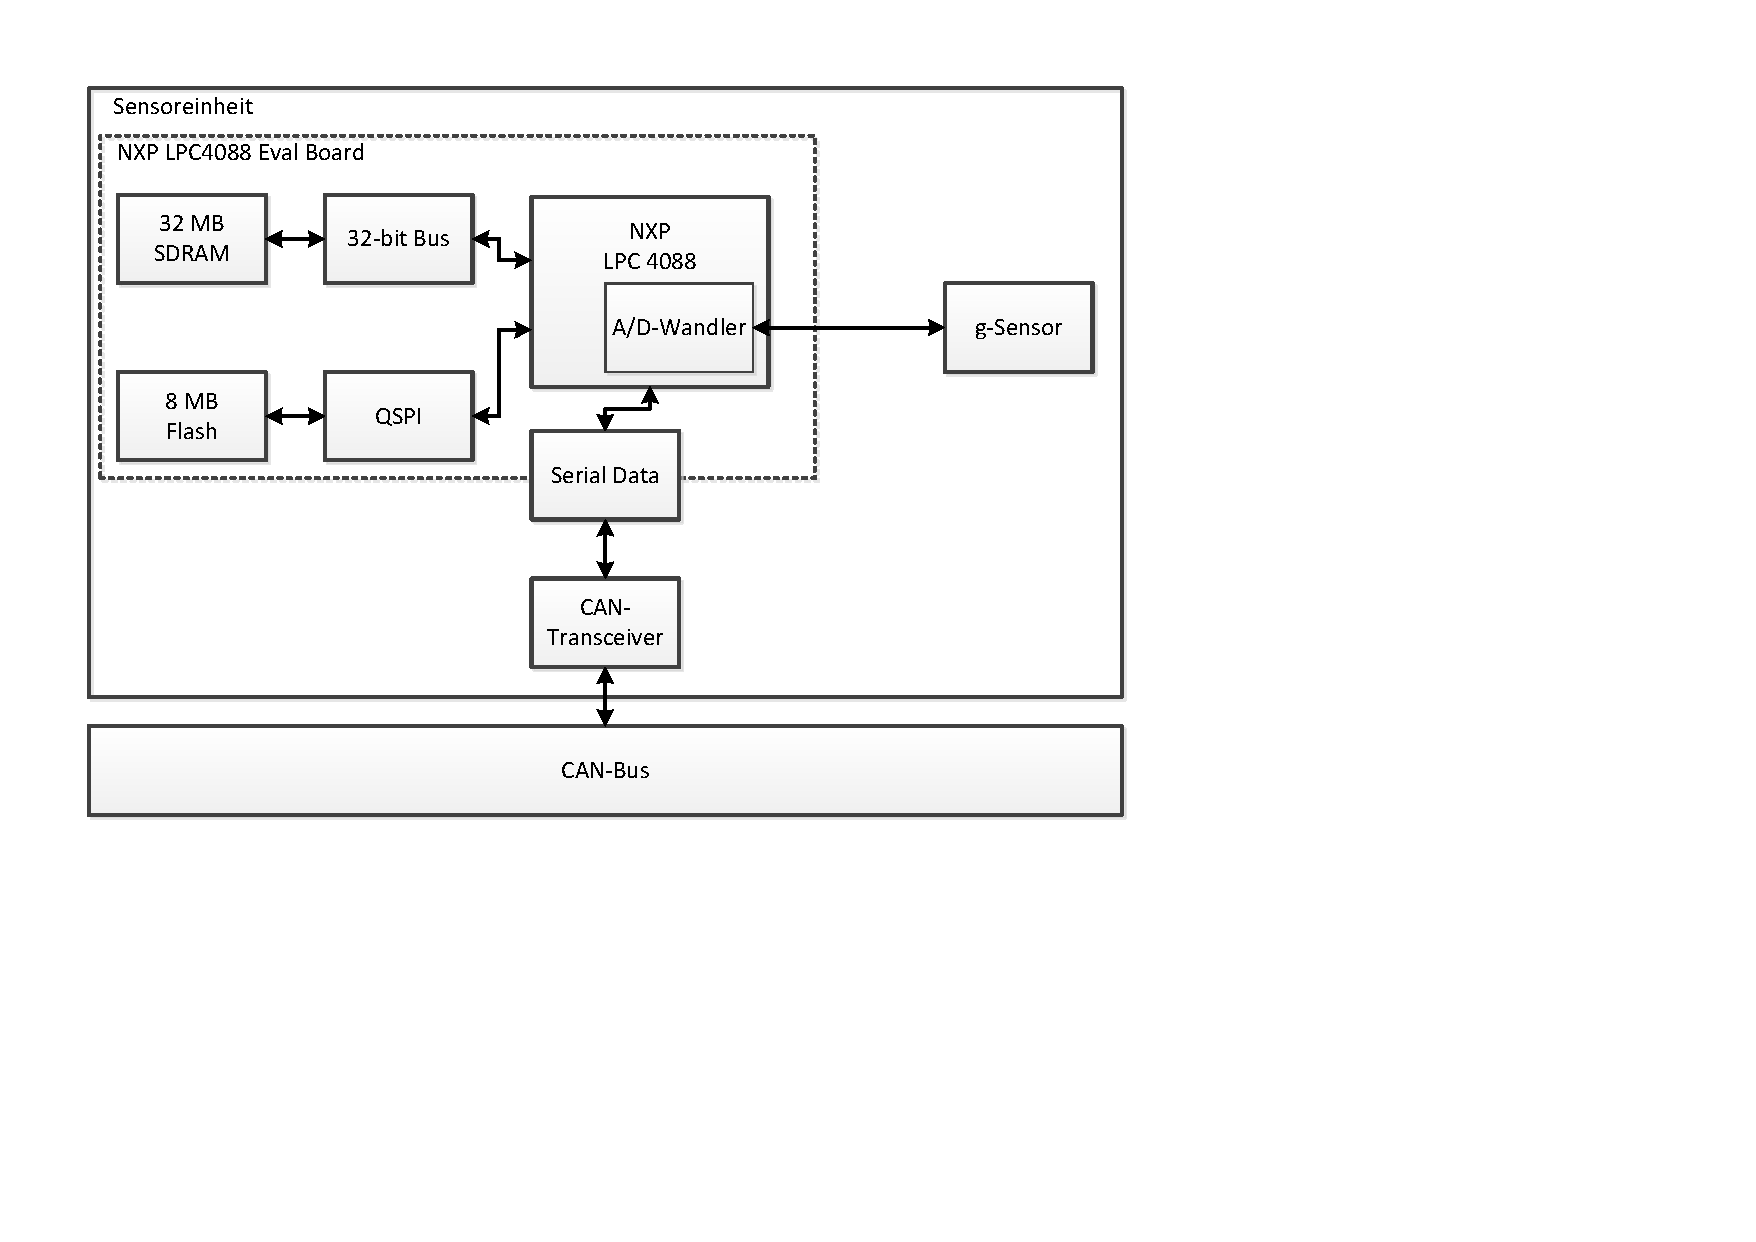
\includegraphics[width=0.8\textwidth]{images/visio/hardware_sensor.pdf}
	\caption{Schematischer Hardware-Aufbau der \gls{sensoreinh}.}
	\label{fig.hw_sensor}
\end{figure}



% !TeX spellcheck = de_CH
%%%%%%%%%%%%%%%%%%%%%%%%%%%%%%%%%%%%%%%%%%%%%%%%%%%%%%%%%%%%%%%%%
%  _____   ____  _____                                          %
% |_   _| /  __||  __ \    Institute of Computitional Physics   %
%   | |  |  /   | |__) |   Zuercher Hochschule Winterthur       %
%   | |  | (    |  ___/    (University of Applied Sciences)     %
%  _| |_ |  \__ | |        8401 Winterthur, Switzerland         %
% |_____| \____||_|                                             %
%%%%%%%%%%%%%%%%%%%%%%%%%%%%%%%%%%%%%%%%%%%%%%%%%%%%%%%%%%%%%%%%%
%
% Project     : BA Welti Keller
% Title       : 
% File        : software.tex Rev. 00
% Date        : 15.09.2014
% Author      : Tobias Welti
%
%%%%%%%%%%%%%%%%%%%%%%%%%%%%%%%%%%%%%%%%%%%%%%%%%%%%%%%%%%%%%%%%%

\chapter{Software-Konzept}\label{chap.software}


\section{Software-Stack}\label{sec.sw_stack}
\todo{Glossar: Impact, Bus, Mikroprozessor, A/D-Wandler, Pin, Sensor, Threshold/Grenzwert, }

\subsection{Überblick}\label{subsec.sw_ueberblick}

\begin{figure}[H]
	\centering
		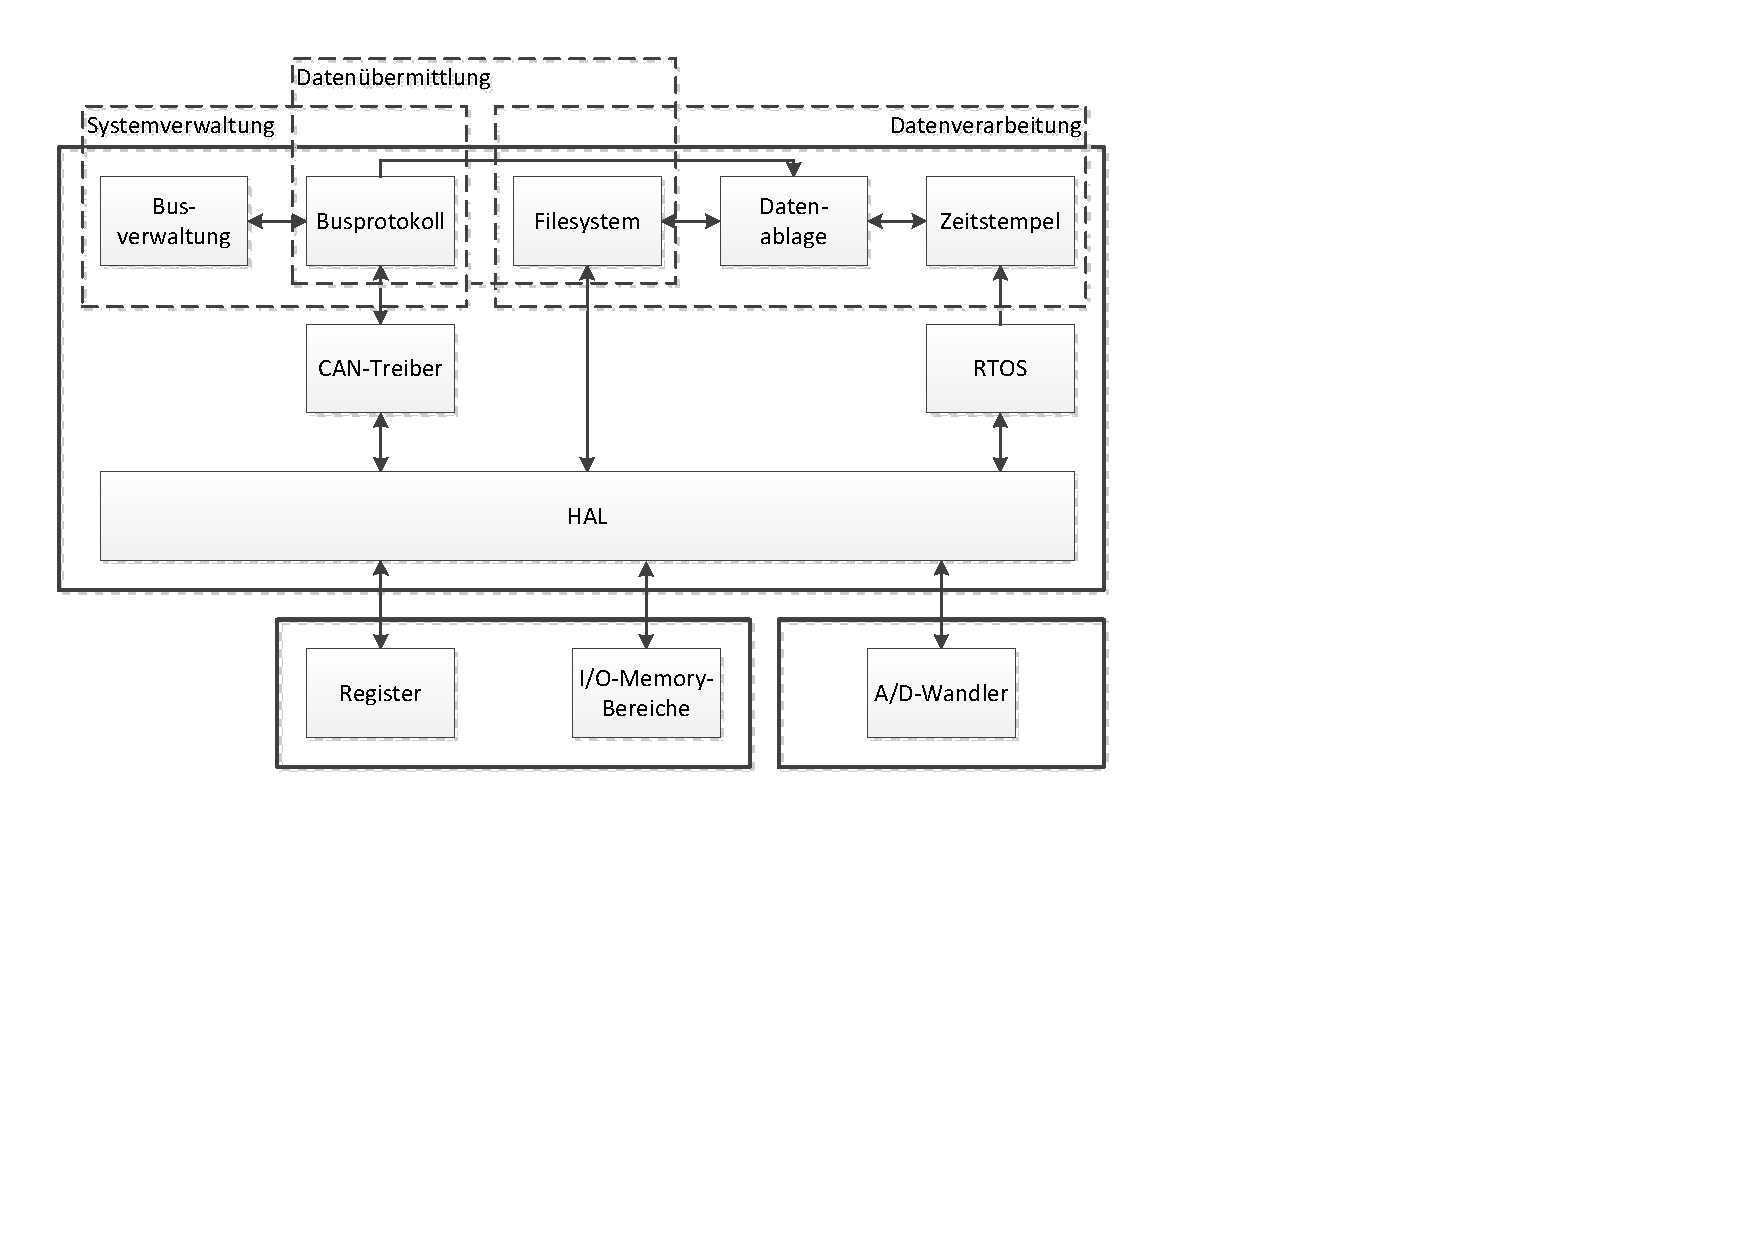
\includegraphics[width=0.8\textwidth]{images/visio/Softwarestack_Logger.pdf}
	\caption{Softwarestack des Datenloggers.}
	\label{fig.sw_logger}
\end{figure}

\begin{figure}[H]
	\centering
		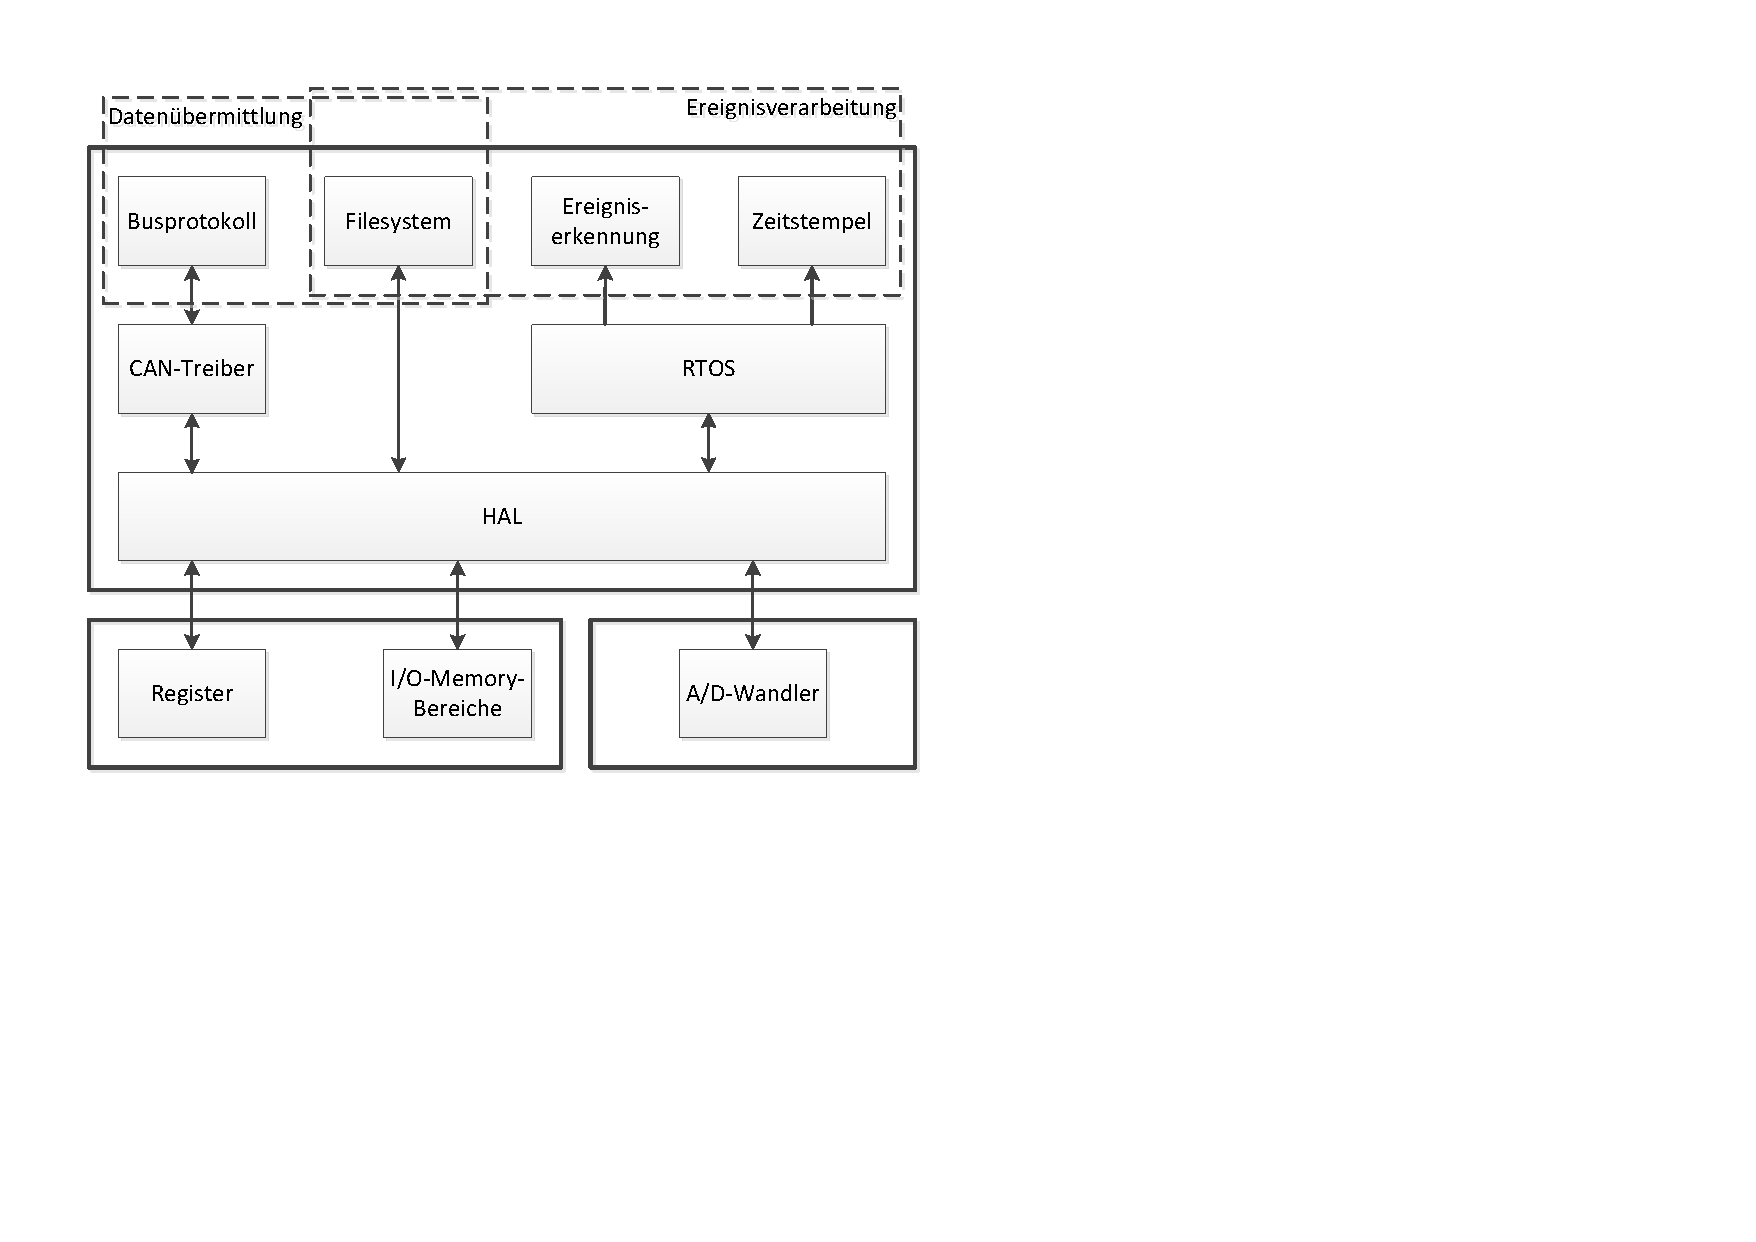
\includegraphics[width=0.8\textwidth]{images/visio/Softwarestack_Sensor.pdf}
	\caption{Softwarestack der Sensoreinheit.}
	\label{fig.sw_sensor}
\end{figure}



\subsection{Messdatenerfassung}\label{subsec.sw_messen}
Der NXP LPC4088 Mikroprozessor verfügt über einen 12-bit A/D-Wandler, der über einen Multiplexer auf acht Pins messen kann. Auf dem verwendeten Quickstart-Board stehen 6 Pins für A/D-Wandlung zur Verfügung. Für die geplante Anwendung reicht ein A/D-Eingang, da der Beschleunigungs-Sensor die Beschleunigung nur auf einer Achse misst. Der A/D-Wandler des NXP LPC4088 wird mit einer Abtastrate von 10~kHz betrieben. Falls höhere Abtastraten nötig sind, kann der A/D-Wandler mit bis zu 400~kHz betrieben werden.



\subsection{Ereigniserkennung}\label{subsec.sw_ereignis}
Vom WSL wurde die Ereigniserkennung bisher mittels Hilbert-Transformation gelöst. Die Hilbert-Transformation liefert die umhüllende Kurve des gemessenen Signals. Überschreitet die Umhüllende den Threshold, markiert dies den Start eines neuen Ereignisses. Fällt die Umhüllende unter den Threshold, ist das Ereignis beendet. Um den Rechenaufwand der Hilbert-Transformation zu umgehen, lösen wir die Ereigniserkennung einfacher.
\todo{FSM-figur anpassen auf neue Stati}
\begin{figure}[H]
	\centering
		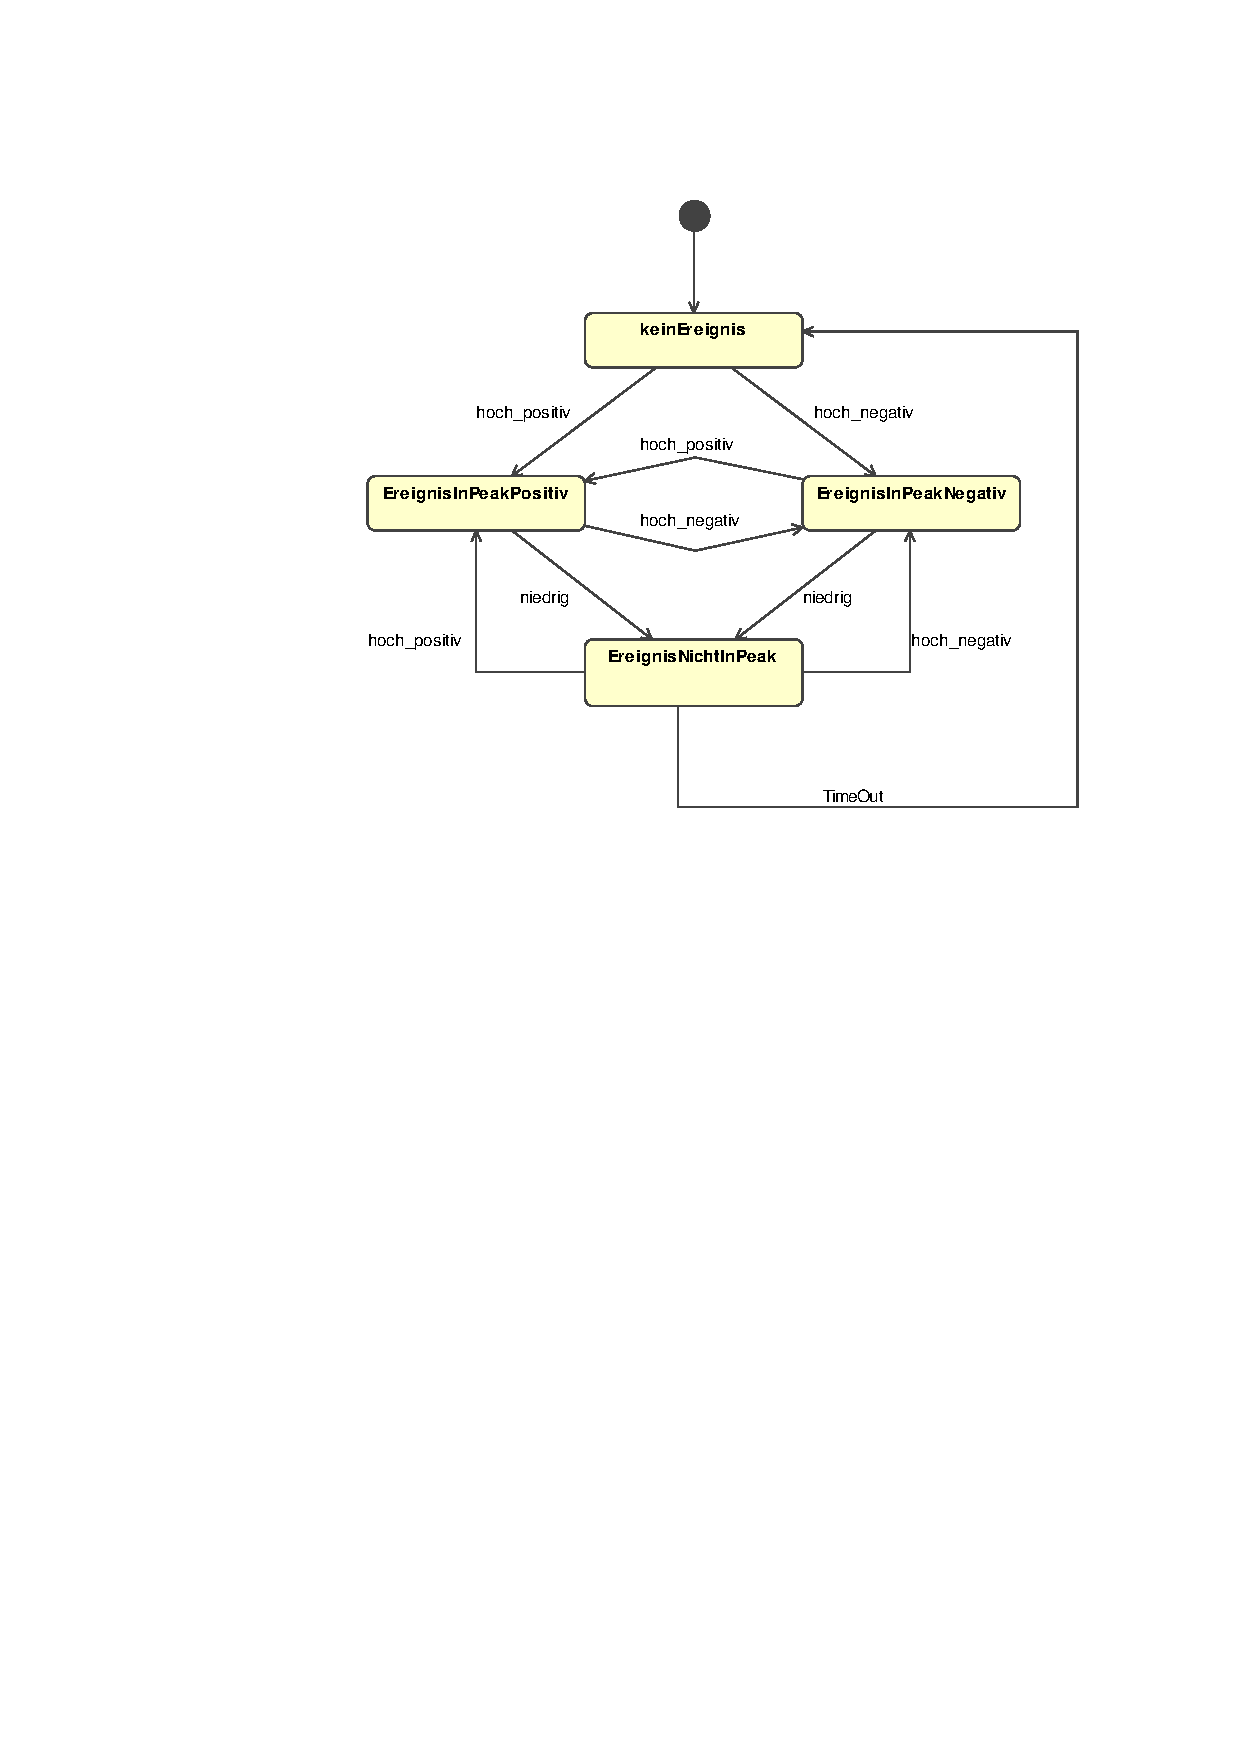
\includegraphics[width=0.6\textwidth]{images/magicdraw/Ereigniserkennung.pdf}
	\caption{Zustandsmaschine der Ereigniserkennung.}
	\label{fig.fsm_impact_detection}
\end{figure}

\todo{Ereigniserkennung beschreiben, welche Parameter können konfiguriert werden}
\todo{Zusammenhänge A/D-Wandlung und Ereigniserkennung und Übertragung beschreiben}
\todo{Verschiedene Betriebsmodi mit Grafiken beschreiben}
\todo{Berechnungen, in welchem Modus wie lange gemessen werden kann, und wie lange ein Sensor mit dem vorhandenen Speicher die Resultate zwischenspeichern kann. Allenfalls ein System erwähnen, das automatisch zwischen verschiedenen Modi hin- und herschalten kann. (Ist allerdings heikel). Wie viele Sensoren können in welchem Modus gleichzeitig am System betrieben werden, bei welcher Ereignisrate ist Schluss mit Busbandbreite.}

\subsection{Timestamp}\label{subsec.sw_timestamp}
\todo{Timestamp beschreiben, Rechnung über die Dauer der eindeutigen Zuweisung.}

\subsection{Verwaltung der Messstation}\label{subsec.sw_busverwaltung}
\todo{Busverwaltung beschreiben}

\begin{figure}[H]
	\centering
		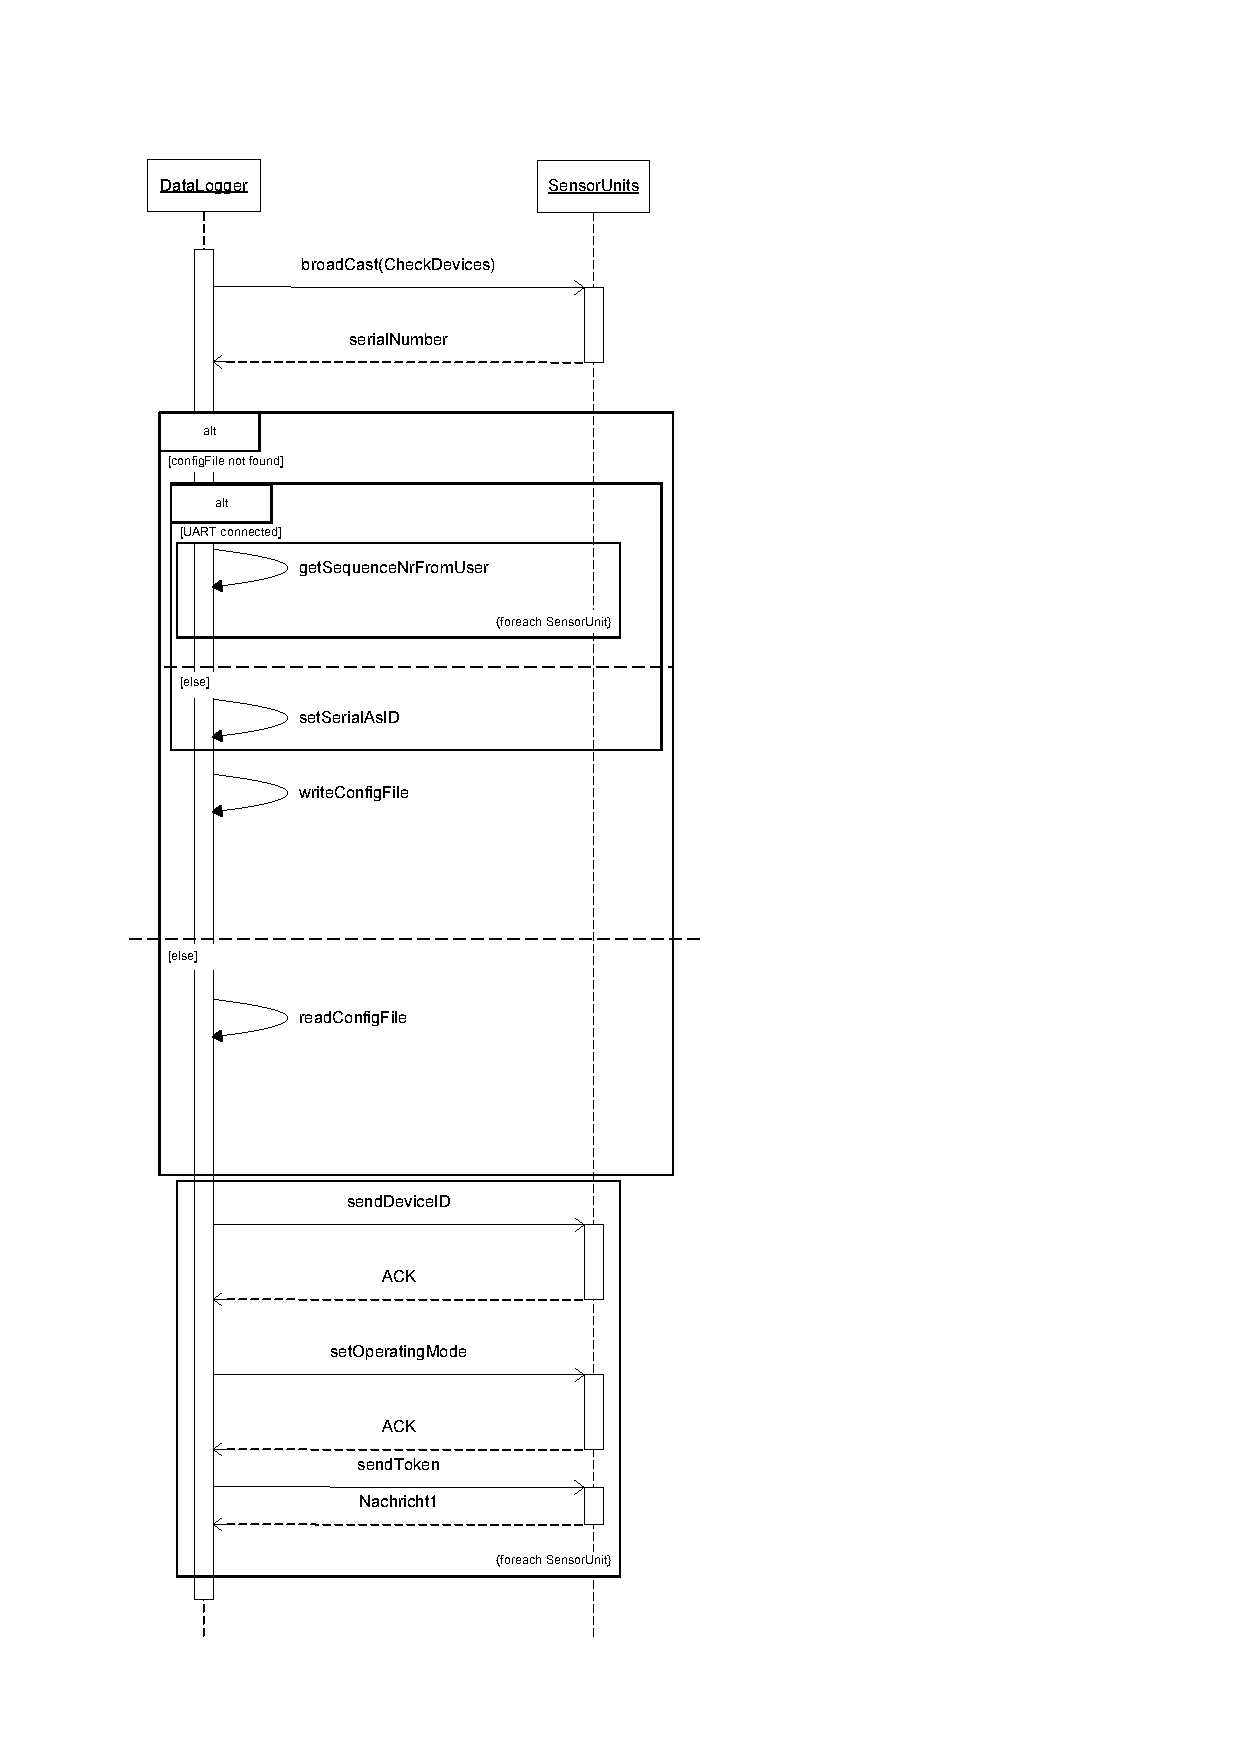
\includegraphics[height=0.9\textheight]{images/magicdraw/StartUpSequenz.pdf}
	\caption{Sequenzdiagramm des Startupvorgangs der Messstation.}
	\label{fig.seq_startup}
\end{figure}

\todo{Figur \ref{fig.seq_startup} aufteilen auf zwei Seiten. (PDF-crop)}

\subsection{Busprotokoll}\label{subsec.sw_busprotokoll}
\todo{Busprotokoll austüfteln. Darstellung siehe HW-Konzept Rioxo, genaue Beschreibung der Nachrichtentypen. Timestamp der einzelnen Peaks bezieht sich auf Offset vom Beginn des Impacts.}
\todo{Kommunikationsdiagramm Bushandler}
\todo{Interrupt-System des Bushandlers aufführen}

\subsection{Filesystem}\label{subsec.sw_filesystem}
\todo{Texten}
\todo{Frage: wird für jeden Sensor ein eigenes File geführt? Kann man alle Files offen lassen oder ist das keine gute Idee? Was ist besser, jedes mal das File-Ende zu suchen um neues anzuhängen?}

\subsection{UART-Kommandozeile}\label{subsec.sw_uart}
\todo{Dokumentation über die Kommandos, wird später für die Bedienungsanleitung gebraucht}

\section{Funktionalität}\label{sec.sw_funktionalitaet}
\todo{Texten}

\section{Konfiguration}\label{sec.sw_konfiguration}
\todo{Hier eine Art Bedienungsanleitung zur Konfiguration geben. Welches Kommando hat was 
zur Folge? (Wird Datenerfassung neu gestartet, werden allenfalls andere Sensoren deaktiviert 
etc.}
% !TeX spellcheck = de_CH
%%%%%%%%%%%%%%%%%%%%%%%%%%%%%%%%%%%%%%%%%%%%%%%%%%%%%%%%%%%%%%%%%
%  _____   ____  _____                                          %
% |_   _| /  __||  __ \    Institute of Computitional Physics   %
%   | |  |  /   | |__) |   Zuercher Hochschule Winterthur       %
%   | |  | (    |  ___/    (University of Applied Sciences)     %
%  _| |_ |  \__ | |        8401 Winterthur, Switzerland         %
% |_____| \____||_|                                             %
%%%%%%%%%%%%%%%%%%%%%%%%%%%%%%%%%%%%%%%%%%%%%%%%%%%%%%%%%%%%%%%%%
%
% Project     : BA Welti Keller
% Title       : 
% File        : resultate.tex Rev. 00
% Date        : 15.09.2014
% Author      : Tobias Welti
%
%%%%%%%%%%%%%%%%%%%%%%%%%%%%%%%%%%%%%%%%%%%%%%%%%%%%%%%%%%%%%%%%%

\chapter{Resultate}\label{chap.resultate}

\section{Testfälle}
Die wichtigsten Testfälle für die grundsätzliche Funktionalität der Messstation konnten erfolgreich abgeschlossen werden. Für einige Tests blieb jedoch nicht genügend Zeit vor der Fertigstellung des Berichts. Diese Tests werden so weit möglich noch nachgeholt.

Im Kapitel \ref{chap.tests} ab Seite \pageref{chap.tests} sind die Testfälle und die Testergebnisse aufgeführt.


Zum Zeitpunkt des Verfassens dieses Berichts konnten keine weiteren Tests durchgeführt werden. Geplant währen

\section{Ereigniserkennung}
Der \gls{adwandler} des \emph{NXP LPC4088} \gls{mc} wurde wie geplant in Betrieb genommen und liefert Messdaten, die sich sehr gut mit dem analogen Ausgangssignal des \gls{sensor}s decken. Abbildung \ref{fig.comparison} zeigt den Vergleich zwischen der Messung von Oszilloskop (blau) und der \gls{sensoreinh} (grün). Die \gls{sensoreinh} arbeitete mit einer \gls{fs} von 10000~\ensuremath{Hz}, das Oszilloskop zeichnete mit einer \gls{fs} von 3.125~MHz auf. Um ein Ereignis zu simulieren, wurde ein Golfball auf den Testaufbau (siehe im Verzeichnis Fotos/Testaufbau/ auf der beiliegenden CD) fallen gelassen. Der Vergleich zeigt, dass die beiden Kurven gut übereinstimmen. 

\begin{figure}
	\centering
		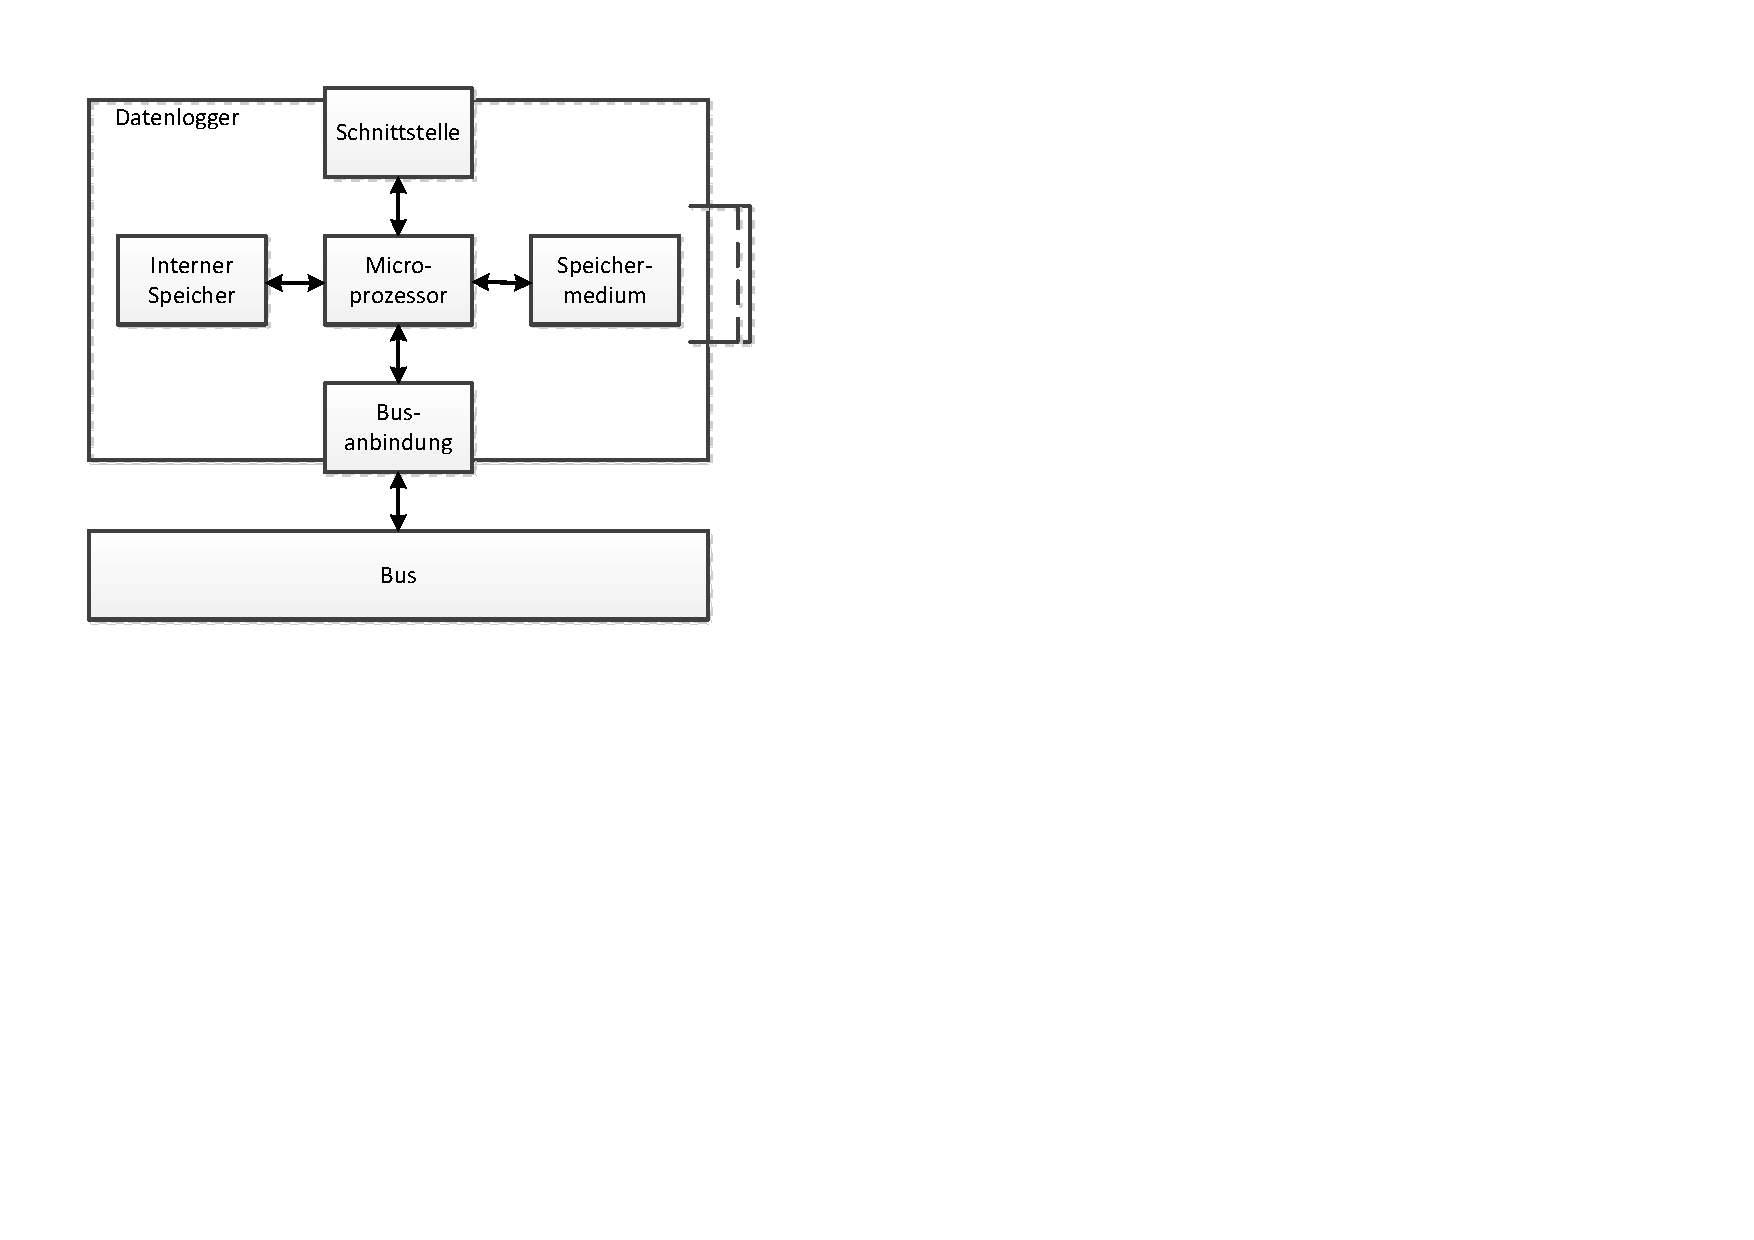
\includegraphics[width=0.8\textwidth]{images/visio/hardwarekonzept_logger.pdf}
	\caption{Vergleichsmessung mit Oszilloskop und \gls{sensoreinh}.}
	\label{fig.comparison}
\end{figure}


Der Betrieb mit 10000~Hz war für unseren Testaufbau genügend, die Peaks traten mit einer Frequenz von ungefähr 2000~Hz auf. Die Frequenz der Peakspitzen variiert sowohl mit der Plattenkonstruktion als auch mit der Korngrösse, Kornbeschaffenheit und der Art des Aufschlags. Daher muss für den tatsächlichen Messbetrieb eine Kalibrierung gemacht werden, um die geeigneten Parameter zu finden.

Für Versuche mit verschiedenen \gls{fs} blieb keine Zeit mehr. So können wir zur Zeit nicht sagen, was die höchstmögliche \gls{fs} mit der aktuellen Software ist.

\section{Daten-Reduktion und -Speicherung}
Die Datenreduktion durch Wahl der verschiedenen Detail-Level ist effizient gelöst und sehr effektiv. Pro Messwert müssen lediglich zwei Vergleiche für die Bestimmung des Signalpegels gemacht werden, sowie zwei Vergleiche mit je einem vorhergehenden Wert für die Bestimmung des Peak-Maximums und des Ereignis-Maximums.

Die Wahl des Detail-Levels beeinflusst lediglich, welche Daten übertragen werden. Auf die Zwischenspeicherung hat sie keinen Einfluss. Vor und nach der Übertragung finden keine komplexen Umrechnungen an den Messdaten statt. Die \gls{bitbreite} wird von 12 Bit auf 8 Bit reduziert. Die grösste Datenreduktion erfolgt durch die Auswahl der relevanten Daten.

\subsection{Rohdaten (raw)}
Es werden alle Messpunkte übertragen und gespeichert. Es findet keine Datenreduktion statt. Pro Messpunkt fällt 1 Byte an. Bei einer \gls{fs} von 10000~Hz resultiert ein Datenstrom von 10000~Byte/s.

\subsection{Detaillierte Ereignisdaten (detailed)}
Es werden nur die Messpunkte der Ereignisse gespeichert. Messpunkte, die nicht zu einem Ereignis gehören, werden verworfen. Der Datenstrom variiert daher mit der Häufigkeit der Ereignisse. Liegt zu 10 \% der Messzeit ein Ereignis vor, wird dies von der \gls{wsl} als hohes Geschiebeaufkommen eingestuft. Eine solche Periode kann über mehrere Stunden anhalten, ist aber nicht jeden Tag zu erwarten.

Bei 10 \% Ereigniszeit wird in diesem Modus eine Datenreduktion um 90 \% erzielt. Für die durchschnittliche Ereigniszeit nehmen wir 5 \% an. Dann resultiert pro \gls{sensor} ein Datenstrom von 500~Byte/s.

\subsection{Peaks (peaks only)}
Der Timestamp, die Dauer des Ereignisses, die Anzahl \glspl{peak} und alle Peakspitzen werden gespeichert. Pro Ereignis fallen 8 Byte an für die Eckdaten und 2 Byte pro Peak. Ein Ereignis hat im Normalfall weniger als 20 Peaks. Wir nehmen somit 48 Byte pro Ereignis an. Bei einem Ereignis pro Sekunde resultiert ein Datenstrom von rund 50 Byte/s.

\subsection{Minimale Daten (sparse)}
Es werden nur der Timestamp, die Dauer des Ereignisses, die Anzahl \glspl{peak} und der maximale Ausschlag des Ereignisses übertragen, das sind 8 Byte pro Ereignis. Der Datenstrom erreicht so lediglich 8 Byte/s.

\subsection{Messdauer}
Je nach Modus fallen sehr unterschiedliche Datenströme pro Sensor an. Ein Vergleich, wie lange mit einem GByte Speicherplatz gemessen werden kann, ist in Tabelle \ref{table.datarate} aufgeführt. Anhand dieser Werte kann abgeschätzt werden, wie lange eine Messstation ohne Wechsel des Speichermediums betrieben werden kann.

\begin{table}
\begin{tabular}{|l|l|l|}
\hline \textbf{Detail-Level} & \textbf{Byte/s} & Messzeit/GByte\\ 
\hline raw                   & 10000 & 27~h \\
\hline detailed              &   500 & 23~d \\
\hline peaks only            &    50 & 231~d \\
\hline sparse                &     8 & 3.9~yr \\
\hline 
\end{tabular}
\caption{Vergleich des Datenaufkommens verschiedener Detail-Levels.}
\label{table.datarate}
\end{table} 

\section{Hardware}
Für den Datenlogger und die Sensoreinheiten wurde mit der Hilfe von Erich Ruff (ZHAW InES) und Valentin Schlatter (ZHAW InES) eine Leiterplatte entworfen sowie Gehäuse gebaut. Die Leiterplatte wurde so entworfen, dass über die Bestückung entschieden wird, ob ein Datenlogger oder eine Sensoreinheit gebaut wird. Für einen Datenlogger wird die Leiterplatte mit einem SD-Karten-Slot bestückt. Für die Sensoreinheit wird ein Tiefpassfilter und der Anschluss für den Sensor bestückt. Beide Varianten enthalten die Spannungsversorgung (12~V auf 5~V), einen CAN-Transceiver und die Anschlüsse für die Kabel. Der Schaltplan und das Leiterplattenlayout befinden sich im Anhang \ref{app.pcb}
% !TeX spellcheck = de_CH
%%%%%%%%%%%%%%%%%%%%%%%%%%%%%%%%%%%%%%%%%%%%%%%%%%%%%%%%%%%%%%%%%
%  _____   ____  _____                                          %
% |_   _| /  __||  __ \    Institute of Computitional Physics   %
%   | |  |  /   | |__) |   Zuercher Hochschule Winterthur       %
%   | |  | (    |  ___/    (University of Applied Sciences)     %
%  _| |_ |  \__ | |        8401 Winterthur, Switzerland         %
% |_____| \____||_|                                             %
%%%%%%%%%%%%%%%%%%%%%%%%%%%%%%%%%%%%%%%%%%%%%%%%%%%%%%%%%%%%%%%%%
%
% Project     : BA Welti Keller
% Title       : 
% File        : diskussion.tex Rev. 00
% Date        : 15.09.2014
% Author      : Tobias Welti
%
%%%%%%%%%%%%%%%%%%%%%%%%%%%%%%%%%%%%%%%%%%%%%%%%%%%%%%%%%%%%%%%%%

\chapter{Diskussion}\label{chap.diskussion}
\todo{Diskussion}
\todo{haben wir erfüllt?, wo gabs schwierigkeiten?, worauf sind wir stolz
, was könnte man jetzt weiter noch machen?
, was ist noch geplant?}



\chapter{Verzeichnisse}\label{chap.verzeichnisse}
 %%%%%%%%%%%%%%%%%%%%%%%%%%%%%%%%%%%%%%%%%%%%%%%%%%%%%%%%%%%%%%%%%
%  _____   ____  _____                                          %
% |_   _| /  __||  __ \    Institute of Computitional Physics   %
%   | |  |  /   | |__) |   Zuercher Hochschule Winterthur       %
%   | |  | (    |  ___/    (University of Applied Sciences)     %
%  _| |_ |  \__ | |        8401 Winterthur, Switzerland         %
% |_____| \____||_|                                             %
%%%%%%%%%%%%%%%%%%%%%%%%%%%%%%%%%%%%%%%%%%%%%%%%%%%%%%%%%%%%%%%%%
%
% Project     : LaTeX doc Vorlage für Windows ProTeXt mit TexMakerX
% Title       : 
% File        : literatur.tex Rev. 00
% Date        : 23.4.12
% Author      : Remo Ritzmann
% Feedback bitte an Email: remo.ritzmann@pfunzle.ch
%
%%%%%%%%%%%%%%%%%%%%%%%%%%%%%%%%%%%%%%%%%%%%%%%%%%%%%%%%%%%%%%%%%

\begin{thebibliography}{99}
\addcontentsline{toc}{section}{Literaturverzeichnis}\label{cha:literaturverzeichnis}

% How to make a Literaturlist nach www.ieee.org/documents/ieeecitationref.pdf
% Erklärung

%Books
\bibitem{robotvision} B. Klaus and P. Horn, Robot Vision. Cambridge, MA: MIT Press, 1986.
%Einzelne Seiten aus Buch
\bibitem{randompatterns} L. Stein, ">Random patterns,"> in Computers and You, J. S. Brake, Ed. New York: Wiley, 1994, pp. 55-70.



\end{thebibliography}

 \listoffigures
 %\addcontentsline{toc}{section}{(Abbildungsverzeichnis)}
 \listoftables
 %\addcontentsline{toc}{section}{(Tabellenverzeichnis)}
 \printglossary
 %\addcontentsline{toc}{section}{(Glossar)}
 \printglossary[type=acronym]
 %\addcontentsline{toc}{section}{(Abkürzungen)}
 \lstlistoflistings
 %\addcontentsline{toc}{section}{(Listingverzeichnis)}
 
% !TeX spellcheck = de_CH
%%%%%%%%%%%%%%%%%%%%%%%%%%%%%%%%%%%%%%%%%%%%%%%%%%%%%%%%%%%%%%%%%
%  _____   ____  _____                                          %
% |_   _| /  __||  __ \    Institute of Computitional Physics   %
%   | |  |  /   | |__) |   Zuercher Hochschule Winterthur       %
%   | |  | (    |  ___/    (University of Applied Sciences)     %
%  _| |_ |  \__ | |        8401 Winterthur, Switzerland         %
% |_____| \____||_|                                             %
%%%%%%%%%%%%%%%%%%%%%%%%%%%%%%%%%%%%%%%%%%%%%%%%%%%%%%%%%%%%%%%%%
%
% Project     : BA Welti Keller
% Title       : 
% File        : anhang.tex Rev. 00
% Date        : 15.09.2014
% Author      : Tobias Welti
%
%%%%%%%%%%%%%%%%%%%%%%%%%%%%%%%%%%%%%%%%%%%%%%%%%%%%%%%%%%%%%%%%%


\pagenumbering{Roman}

\appendix
\chapter{Anhang}\label{chap.anhang}



\section{Projektmanagement}\label{sec.projektmanagement}

\begin{itemize}
\item Offizielle Aufgabenstellung, Projektauftrag
\item (Zeitplan)
\item (Besprechungsprotokolle oder Journals)
\end{itemize}



\section{Weiteres}\label{weiteres}

\begin{itemize}
\item CD mit dem vollständigen Bericht als pdf-File inklusive Film- und Fotomaterial
\item (Schaltpläne und Ablaufschemata)
\item (Spezifikationen u. Datenblätter der verwendeten Messgeräte und/oder Komponenten)
\item (Berechnungen, Messwerte, Simulationsresultate)
\item (Stoffdaten)
\item (Fehlerrechnungen mit Messunsicherheiten)
\item (Grafische Darstellungen, Fotos)
\item (Datenträger mit weiteren Daten (z.B. Software-Komponenten) inkl. Verzeichnis der auf diesem Datenträger abgelegten Dateien)
\item (Softwarecode)
\end{itemize}



\end{document}
